\pagenumbering{arabic}
%\documentclass[slides]{beamer}
\documentclass[mathserif, 8pt]{beamer}
\usepackage[framesassubsections]{beamerprosper}
\setbeamercovered{transparent}
%\documentclass[slides,hyperref={pdfpagelabels=false}]{beamer}
%\documentclass[handout,gray]{beamer}
\usepackage[T1]{fontenc}
\usepackage[utf8]{inputenc}
\usepackage{textcomp}
\usepackage{algorithm}
\usepackage{algorithmic}
\usepackage{color}
\usepackage{verbatim}
\usepackage{amsbsy}
\usepackage{multirow}
\usepackage{multicol}
\usepackage{booktabs} % Make some nice tables
\usepackage{ae,aecompl}

%%%%%%%%%%%% COULEURS %%%%%%%%%%%%%%%%%%%%%%%%%%%

\mode<presentation>
{
  \definecolor{beamerstructure}{RGB}{43,79,112}
  \definecolor{sidebackground}{RGB}{230,242,250}
  \definecolor{CTCC}{RGB}{133,188,228}
  \color{beamerstructure}
  \usetheme{default}
  \usepackage{courier}
  \beamertemplateballitem
\setbeamertemplate{navigation symbols}{}
%\setbeamertemplate{sidebar left}{\thispdfpagelabel{\insertframenumber}}
%\setbeamertemplate{footline}{\quad\insertframenumber}
%\usecolortheme{CTCC}
}
\usebackgroundtemplate{
\includegraphics[width=1.02\paperwidth]{../templets/ctcc_general.jpg}}

\title{\\\vspace{1cm}
Density Functional Theory with multiwavelets
}
%\subtitle{\textcolor{magenta}{My subtitle (if applicable)}}
\author{Stig Rune Jensen}
\institute[CTCC]{\\[-6mm]stig.r.jensen@uit.no\\[6mm]UiT - The Arctic University of Norway\\[6mm]

\includegraphics[height=1.5cm]{../templets/uio.pdf}\hspace{1cm} 

\includegraphics[height=1.5cm]{../templets/sff.pdf}\hspace{1cm}

\includegraphics[height=1.5cm]{../templets/uit.pdf}}
\date{Stony Brook, 4 August 2016}

\newcommand{\gb}[1]{green!#1!black}
\newcommand{\rb}[1]{red!#1!black}
\newcommand{\bb}[1]{blue!#1!black}
\newcommand{\coleq}{red!60!black}
\newcommand{\du}{\textrm{d}}

\newcommand{\red}[1]{\textcolor{red}{#1}}

\begin{document}

\footnotesize
\setlength{\unitlength}{\textwidth}

{
\usebackgroundtemplate{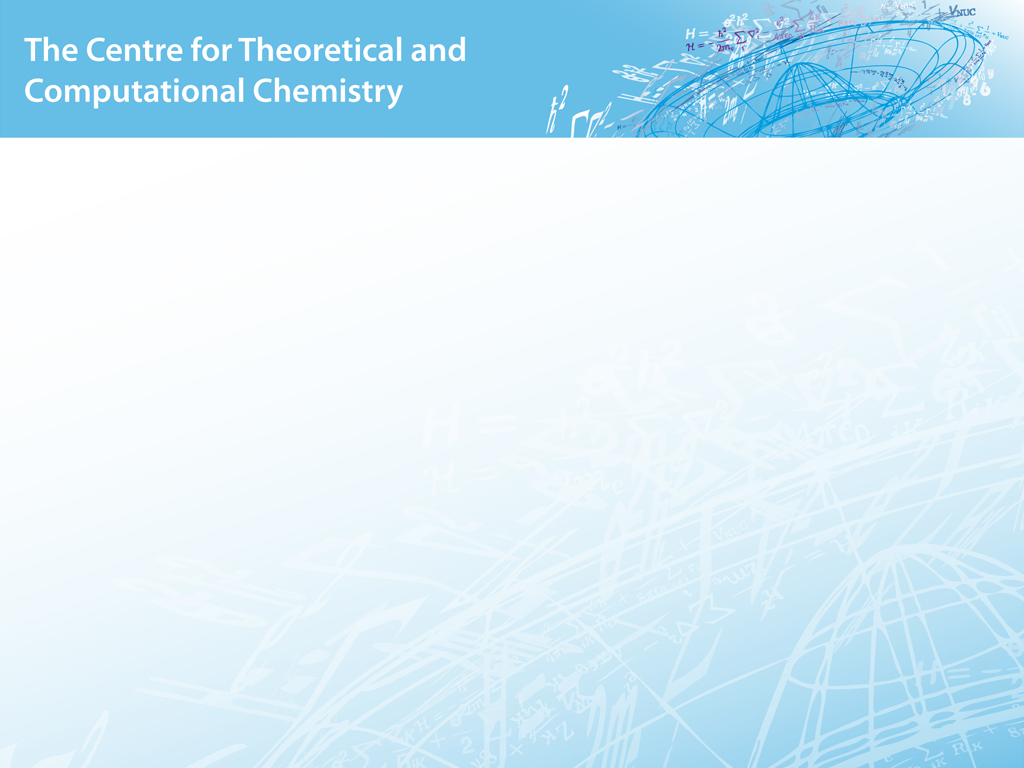
\includegraphics[width=1.02\paperwidth]{../templets/ctcc_forside.jpg}}
\maketitle
}

\begin{frame}
    \frametitle{Outlook}
    \begin{itemize}
	\item   \textbf{Density Functional Theory}
	\begin{itemize}
	    \item General DFT
            \item Hohenberg-Kohn
            \item Kohn-Sham
            \item XC energy and potential
            \item Kohn-Sham equations
            \item Total energy
	    \item Integral reformulation
	\end{itemize}
	\ \\
	\ \\
	\item   \textbf{Iterative algorithms}
	\begin{itemize}
            \item One-electron system
            \item Hydrogen atom
            \item Energy update
            \item KAIN
            \item Many-electron systems
            \item Fock/KS operator
            \item Orthonormalizations
            \item Fock matrix without kinetic operator
            \item Total energy without kinetic operator
            \item Orbital localization
            \item Lambda update
            \item Quadratic energy
            \item Final algorithm
	\end{itemize}
    \end{itemize}
\end{frame}

\begin{frame}
    \frametitle{The molecular Schr\"{o}dinger equation}
    \ \\
    \begin{equation}
	\nonumber
	\hat{H}\psi = E\psi
    \end{equation}
    \ \\
    \begin{equation}
	\nonumber
	\hat{H} =   -\sum_I \frac{\nabla^2}{2M_I} - \sum_i \frac{\nabla^2}{2}
		    +\sum_{I>J} \frac{Z_IZ_J}{|\boldsymbol{R}_I-\boldsymbol{R}_J|} 
		    -\sum_{i,I} \frac{Z_I}{|\boldsymbol{r}_i-\boldsymbol{R}_I|} 
		    +\sum_{i>j} \frac{1}{|\boldsymbol{r}_i-\boldsymbol{r}_j|} 
    \end{equation}
    \ \\
    \ \\
    \ \\
    \centering
    For an $N$-particle problem, the wave function is $3N$-dimensional
    \begin{equation}
	\nonumber
	\psi = \psi(\boldsymbol{r}_1,\boldsymbol{r}_2,\dots,\boldsymbol{r}_N)
    \end{equation}
    \ \\
    \ \\
    \ \\
    \pause
    \centering
    $\beta$-Carotene ($C_{40}H_{56}$) has 296 electrons and an 888-dimensional
    electronic wavefunction!
    \only<1>{
    \begin{center}
    %white background
    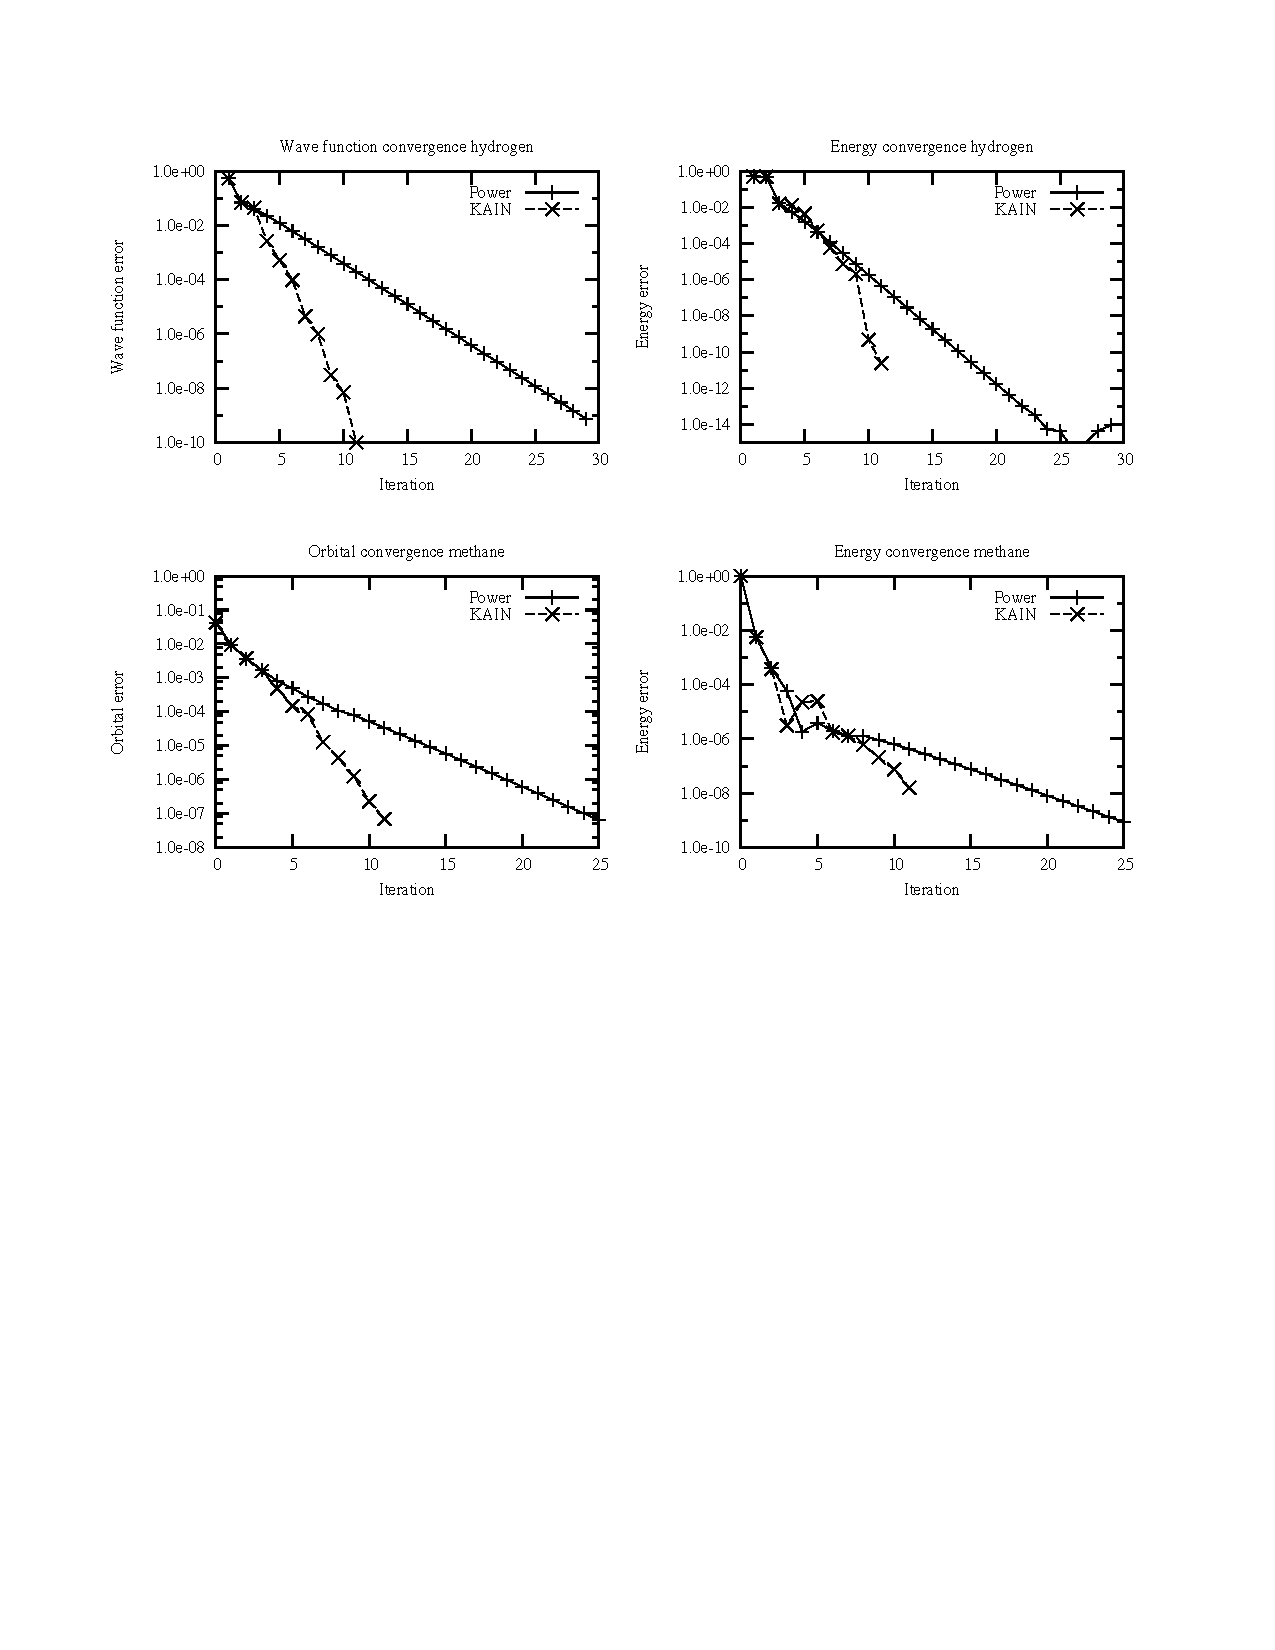
\includegraphics[scale=0.3, clip, viewport = 0 0 900 280]{figures/convergence.pdf}
    \end{center}
    }
    \only<2>{
    \begin{center}
    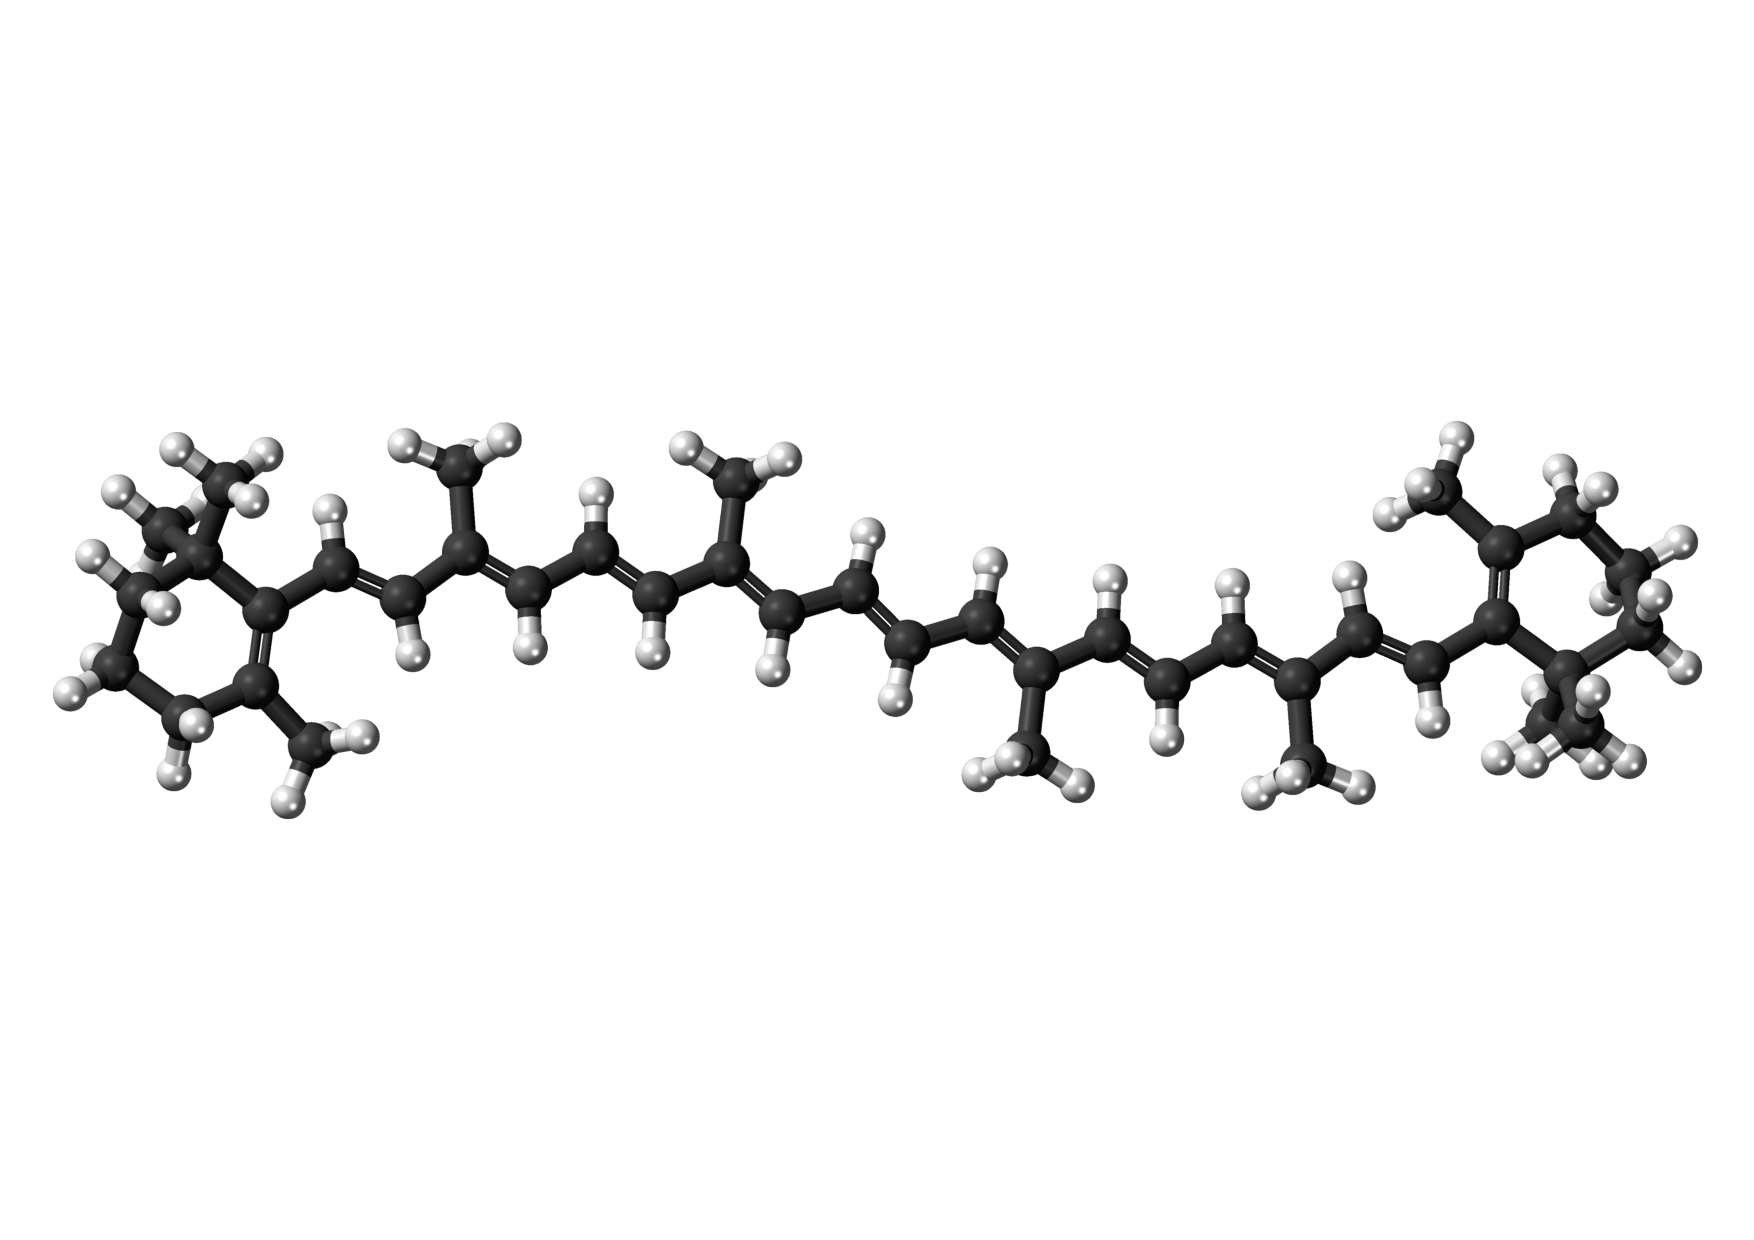
\includegraphics[scale=0.3, clip, viewport = 0 150 900 430]{figures/beta-carotene.pdf}
    \end{center}
    }
\end{frame}

\begin{frame}
    \frametitle{Density Functional Theory}
    \centering
    Dramatically reduce the dimensionality
    \begin{equation}
	\nonumber
	\rho(\boldsymbol{r}_1) = N \int |\psi(\boldsymbol{r}_1, \boldsymbol{r}_2,\dots,
	\boldsymbol{r}_N)|^2 d\boldsymbol{r}_2\cdots d\boldsymbol{r}_N
    \end{equation}
    \ \\
    \ \\
    \ \\
    \pause
    Energy expressed as functional of the density
    \begin{equation}
	\nonumber
	E[\rho] = T_s[\rho] + V_{ne}[\rho] + J[\rho] + E_{xc}[\rho]
    \end{equation}
    \ \\
    \ \\
    \ \\
    \begin{columns}
    \begin{column}{.50\textwidth}
    \centering
    \pause
    \textbf{Energy expressions}
    \begin{align}
	\nonumber
	V_{ne}[\rho]	&= \int \rho(\boldsymbol{r})v_{nuc}(\boldsymbol{r})d\boldsymbol{r}\\
	\nonumber
			&\\
	\nonumber
	J[\rho] &= \frac{1}{2} \int \rho(\boldsymbol{r})v_{el}(\boldsymbol{r})d\boldsymbol{r}\\
	\nonumber
			&\\
	\nonumber
	E_{xc}[\rho]	&= \int F_{xc}(\rho) d\boldsymbol{r}
    \end{align}
    \end{column}
    \begin{column}{.50\textwidth}
    \centering
    \pause
    \textbf{Potentials}
    \begin{align}
	\nonumber
	v_{nuc}(\boldsymbol{r}) &= -\sum_I\frac{Z_I}{|\boldsymbol{r}-\boldsymbol{R}_I|}\\
	\nonumber
			&\\
	\nonumber
	v_{el}(\boldsymbol{r}) &= 
	    \int \frac{\rho(\boldsymbol{r}')}{4\pi|\boldsymbol{r}-\boldsymbol{r}'|} d\boldsymbol{r}'\\
	\nonumber
			&\\
	\nonumber
	v_{xc}(\boldsymbol{r}) &= \frac{\delta E_{xc}[\rho]}{\delta\rho}
    \end{align}
    \end{column}
    \end{columns}    
\end{frame}

\begin{frame}
    \frametitle{Kohn-Sham DFT}
    \centering
    Express density through one-electron orbitals
    \begin{equation}
	\nonumber
	\rho(\boldsymbol{r}) = \sum_i |\phi_i(\boldsymbol{r})|^2
    \end{equation}
    \ \\
    \ \\
    \ \\
    \ \\
    \pause
    \begin{columns}
    \begin{column}{.50\textwidth}
    \centering
    Kinetic energy
    \begin{equation}
	\nonumber
	T_s[\rho] = -\sum_i \frac{1}{2}\nabla^2\phi_i(\boldsymbol{r})
    \end{equation}
    \end{column}
    \begin{column}{.50\textwidth}
    \centering
    Effective potential
    \begin{equation}
	\nonumber
	v_{eff}(\boldsymbol{r}) = v_{nuc}(\boldsymbol{r}) + v_{el}(\boldsymbol{r}) + v_{xc}(\boldsymbol{r})
    \end{equation}
    \end{column}
    \end{columns}
    \ \\
    \ \\
    \ \\
    \ \\
    \pause
    \centering
    \textbf{The Kohn-Sham equations}
    \begin{equation}
	\nonumber
	\left[-\frac{1}{2}\nabla^2 + v_{eff}(\boldsymbol{r})\right]\phi_i(\boldsymbol{r}) = 
	\epsilon_i\phi_i(\boldsymbol{r})
    \end{equation}
\end{frame}

\begin{frame}
    \frametitle{Total energy calculation}
\end{frame}

\begin{frame}
    \frametitle{Computational chemistry}
    \begin{center}
    \only<1>{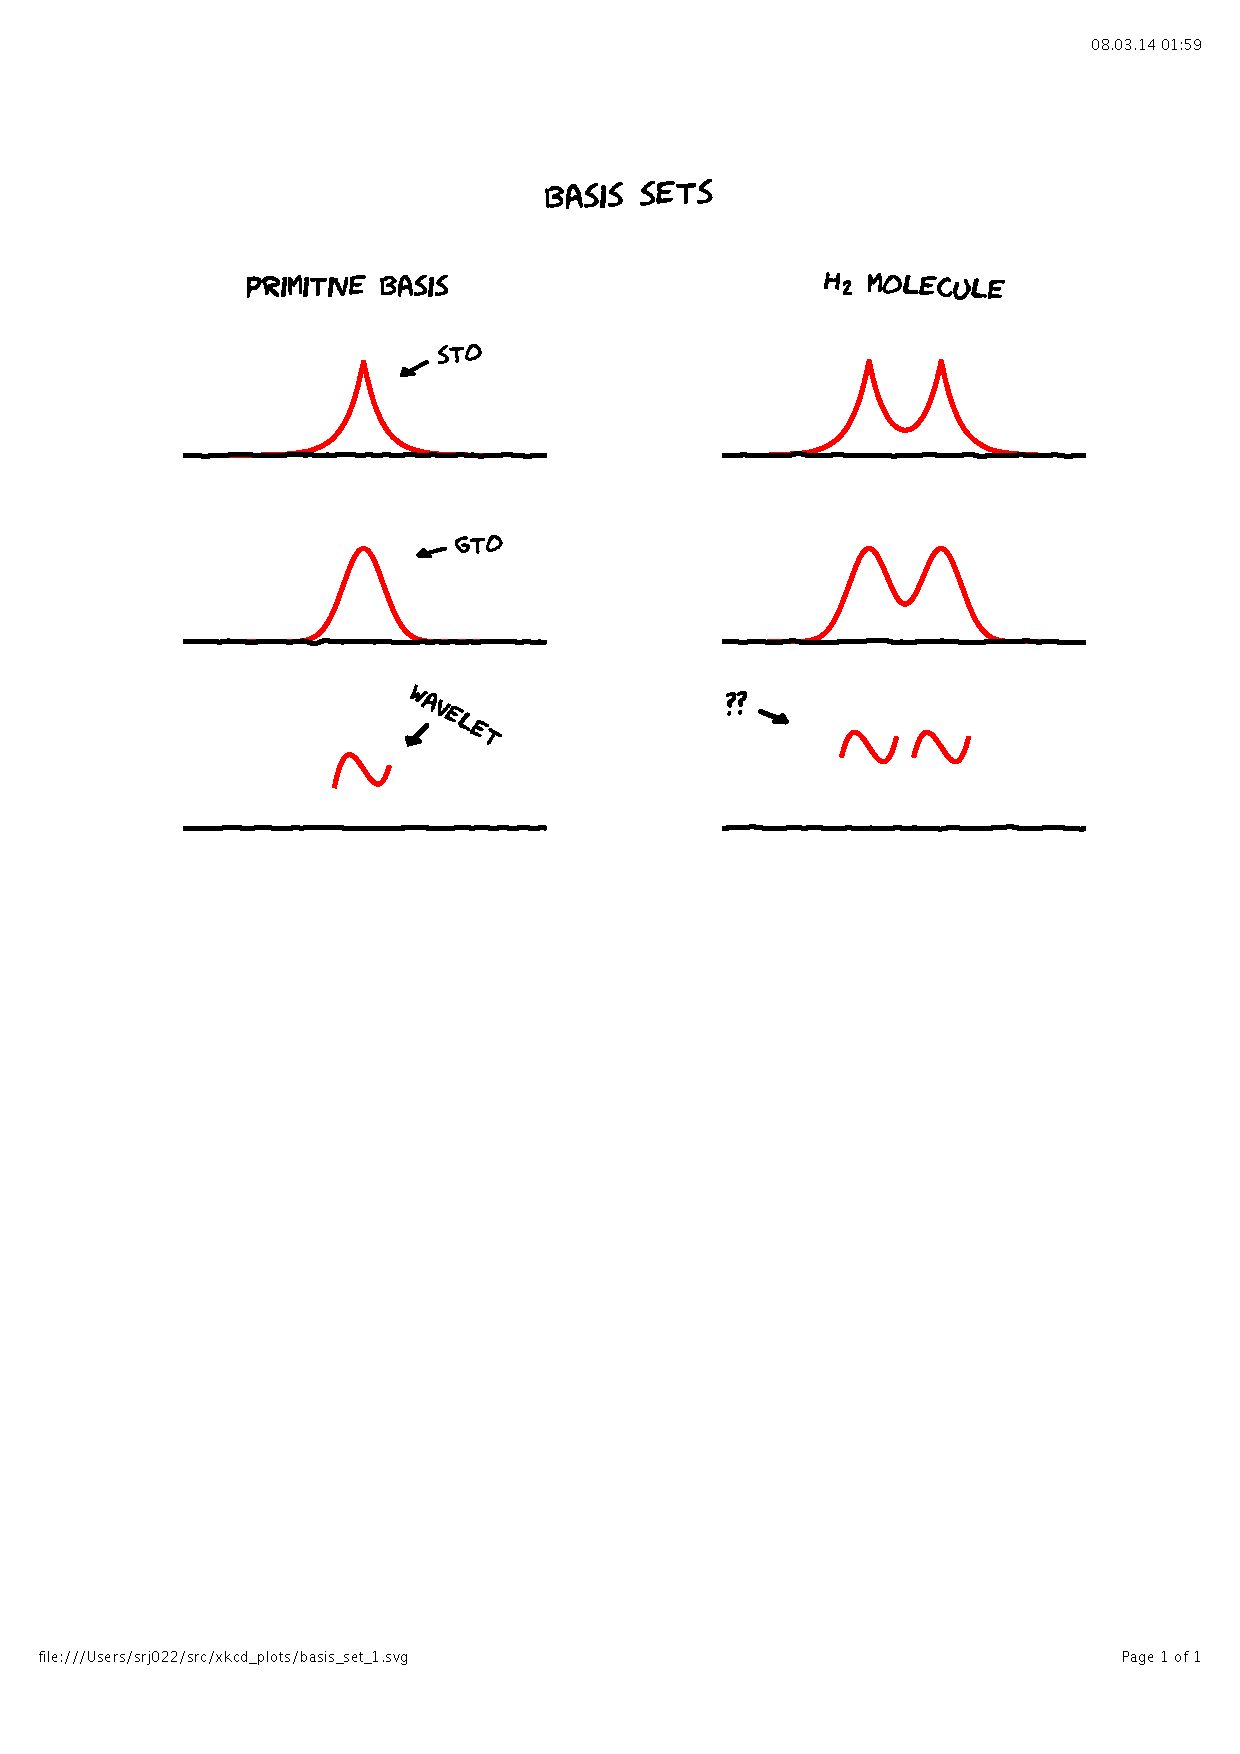
\includegraphics[scale=0.5, clip, viewport = 50 300 550 800]{figures/basis_set_1.pdf}}
    \only<2>{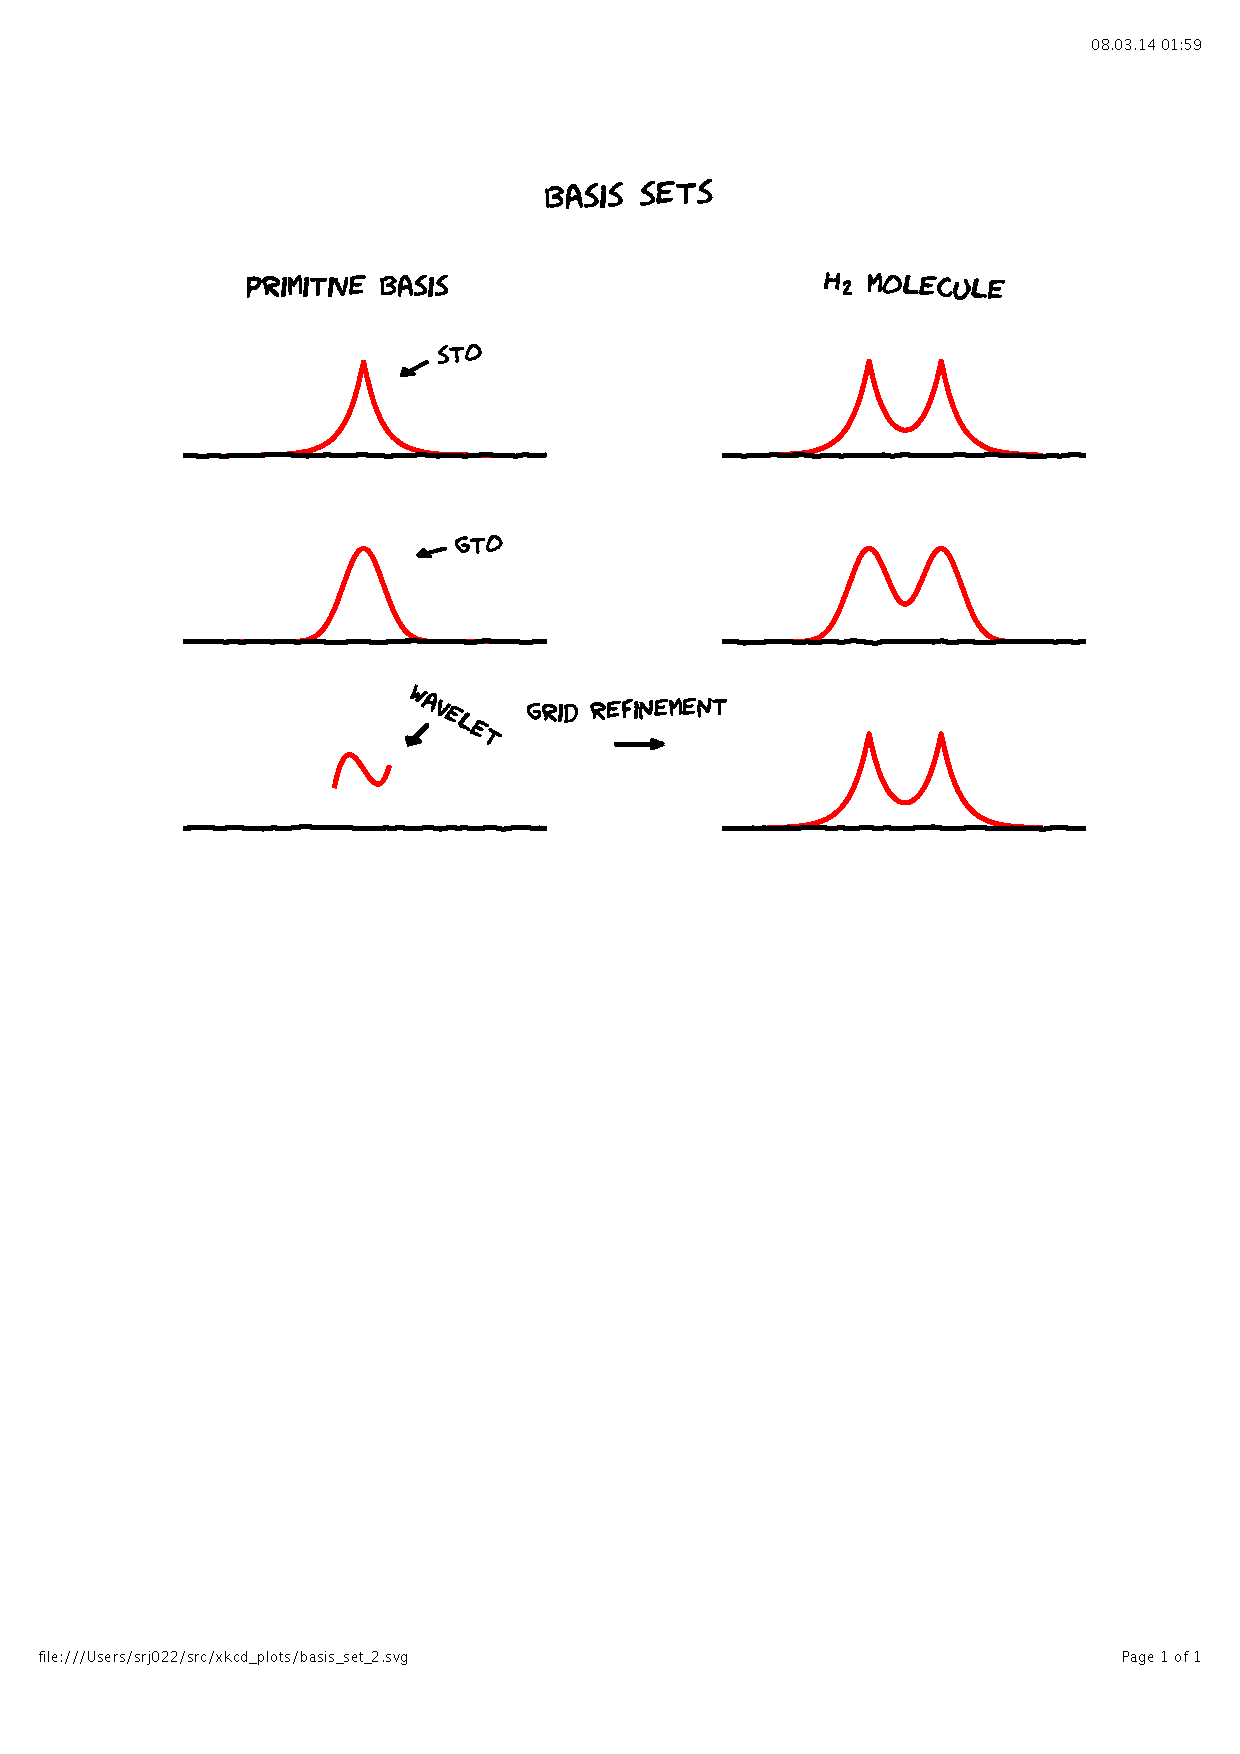
\includegraphics[scale=0.5, clip, viewport = 50 300 550 800]{figures/basis_set_2.pdf}}
    \only<3>{\includegraphics[scale=0.5, clip, viewport = 0 300 550 800]{figures/chemical_accuracy.pdf}}
    \end{center}
\end{frame}

\begin{frame}
    \frametitle{Integral formulation}
    \centering
    The Kohn-Sham equations
    \begin{equation}
	\nonumber
	\left[-\frac{1}{2}\nabla^2 + v_{eff}(\boldsymbol{r})\right]
	\phi_i(\boldsymbol{r}) =\ \epsilon_i \phi(\boldsymbol{r})
    \end{equation}
    \ \\
    \ \\
    \ \\
    \ \\
    \pause
    can be expressed in integral form
    \begin{equation}
	\nonumber
	\phi_i(\boldsymbol{r}) =\ -2\int H^{\mu}(\boldsymbol{r}-\boldsymbol{r}')\
	    \Big[v_{eff}(\boldsymbol{r}') \phi_i(\boldsymbol{r}')\Big] d\boldsymbol{r}'
    \end{equation}
    \ \\
    \ \\
    \ \\
    \ \\
    \pause
    and solved iteratively
    \begin{equation}
	\nonumber
	\phi_i^{n+1} =\ -2\hat{H}\left[v_{eff}^n\phi_i^n\right]
    \end{equation}
    \ \\
    \ \\
    \ \\
    \ \\
    standard iterative subspace acceleration techniques (KAIN or DIIS) can be applied
\end{frame}

\begin{frame}
    \frametitle{Hydrogen atom}
    \centering
    \textbf{Power iteration}
    \begin{equation}
	\nonumber
	\phi^{n+1} = -2\hat{H}\left[v_{nuc}\phi^n\right]
    \end{equation}
    \ \\
    \ \\
    \ \\
    \begin{columns}
    \begin{column}{.10\textwidth}
    \ \\
    \end{column}
    \begin{column}{.40\textwidth}
    \centering
    \textbf{Orbital update}
    \begin{equation}
	\nonumber
	\Delta\phi^n = \phi^{n+1} - \phi^n
    \end{equation}
    \end{column}
    \begin{column}{.50\textwidth}
    \centering
    \textbf{Energy update}
    \begin{equation}
	\nonumber
	\Delta \epsilon^n = \left<\phi^{n+1}|v_{nuc}|\Delta\phi^n\right>
    \end{equation}
    \end{column}
    \end{columns}    
    \begin{center}
	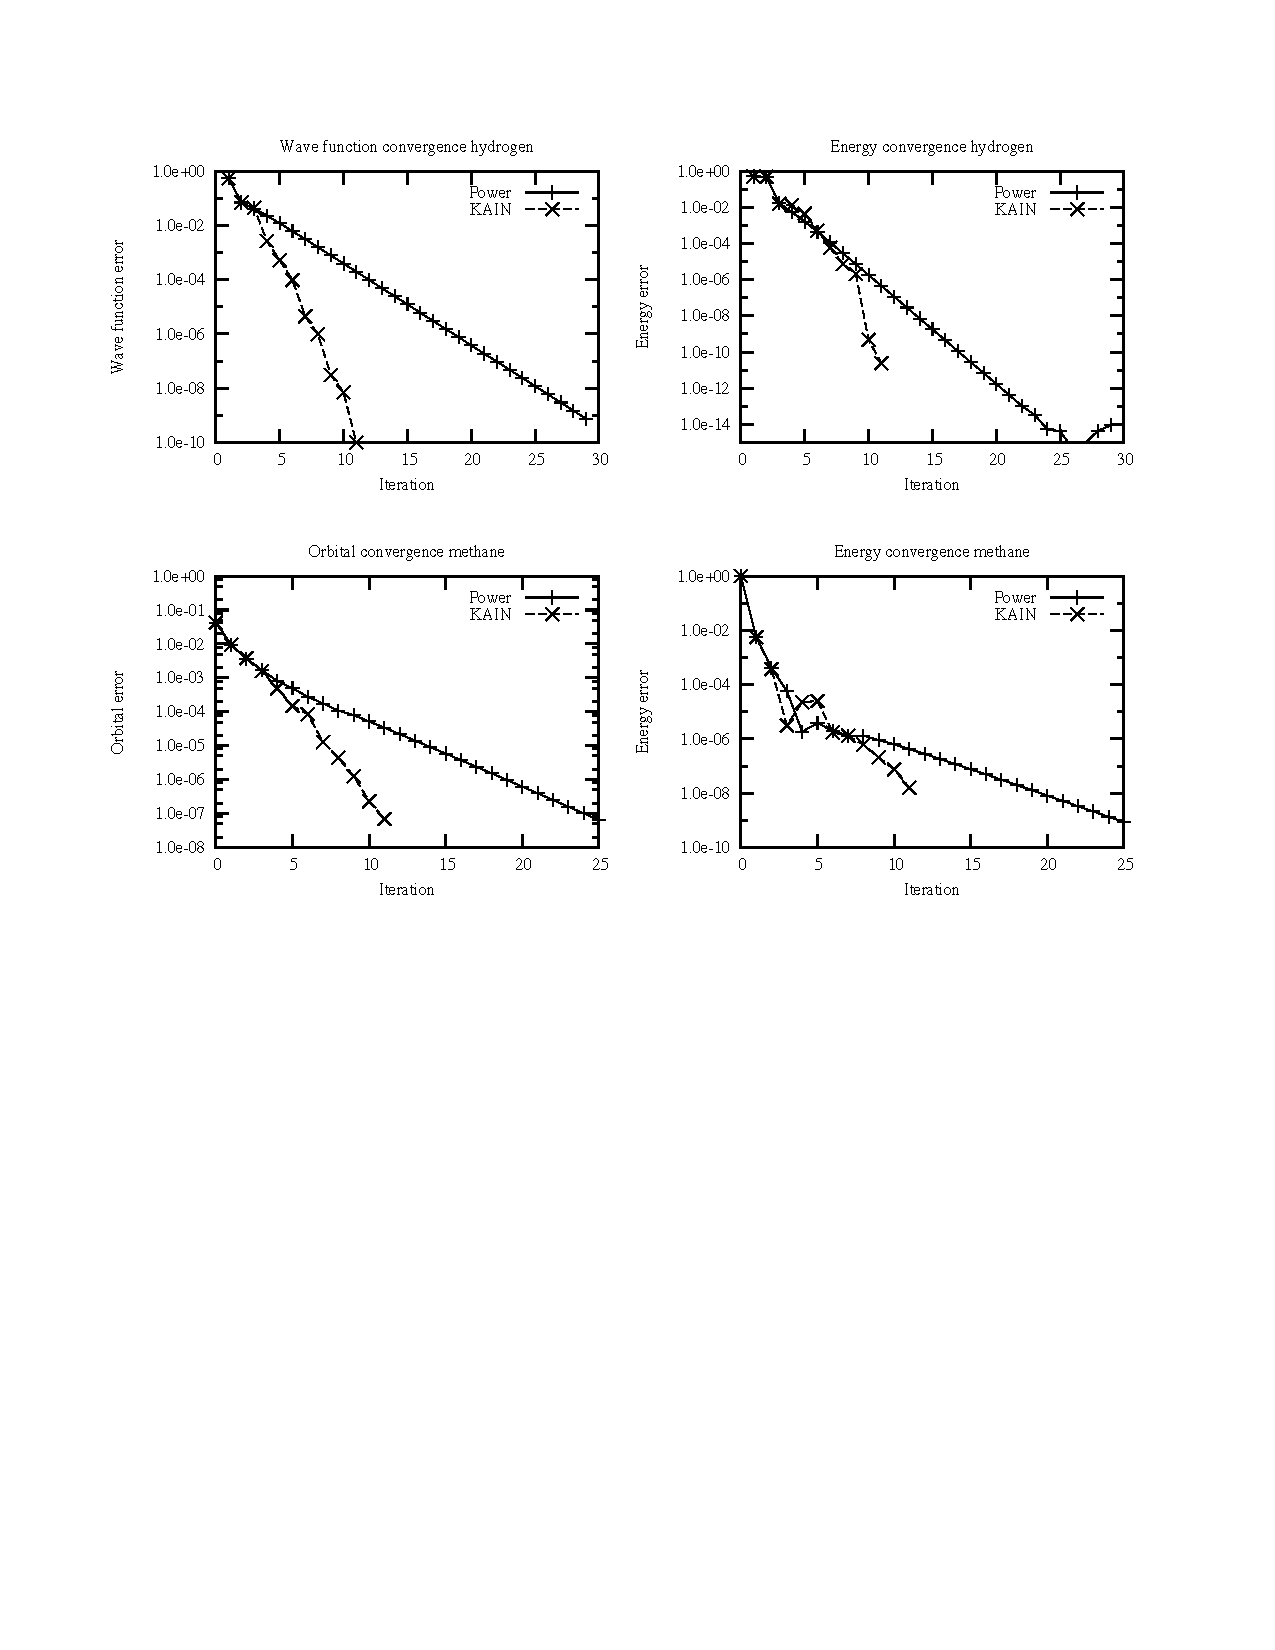
\includegraphics[scale=0.6, clip, viewport = 50 550 540 730]{figures/convergence.pdf}
    \end{center}
\end{frame}

\begin{frame}
    \frametitle{Hydrogen atom}
    \only<1>{\includegraphics[viewport = 50 430 300 640, clip, scale=1.2]{figures/s1Orb_1.pdf}}
    \only<2>{\includegraphics[viewport = 50 430 300 640, clip, scale=1.2]{figures/s1Orb_2.pdf}}
    \only<3>{\includegraphics[viewport = 50 430 300 640, clip, scale=1.2]{figures/s1Orb_3.pdf}}
    \only<4>{\includegraphics[viewport = 50 430 300 640, clip, scale=1.2]{figures/s1Orb_4.pdf}}
    \only<5>{\includegraphics[viewport = 50 430 300 640, clip, scale=1.2]{figures/s1Orb_5.pdf}}
    \only<6>{\includegraphics[viewport = 50 430 300 640, clip, scale=1.2]{figures/s1Orb_10.pdf}}
\end{frame}

\begin{frame}
    \frametitle{Many-electron systems}
    \begin{columns}
    \begin{column}[b]{0.1\textwidth}
    \ \\
    \end{column}
    \begin{column}[b]{0.4\textwidth}
    \centering
    Density
    \begin{equation}
	\nonumber
	\rho^n(\boldsymbol{r}) = \sum_i |\phi_i^n(\boldsymbol{r})|^2
    \end{equation}
    \end{column}
    \begin{column}[b]{0.4\textwidth}
    \centering
    Potentials
    \begin{equation}   
	\nonumber
	\rho^n(\boldsymbol{r}) \rightarrow v_{eff}^n(\boldsymbol{r})
    \end{equation}
    \end{column}
    \begin{column}[b]{0.1\textwidth}
    \ \\
    \end{column}
    \end{columns}
    \ \\
    \ \\
    \begin{columns}
    \begin{column}[b]{0.1\textwidth}
    \ \\
    \end{column}
    \begin{column}[b]{0.4\textwidth}
    \centering
    Power iteration
    \begin{equation}
	\nonumber
	\tilde{\phi}_i^n = -2\hat{H}\left[v_{eff}^n\phi_i^n\right]
    \end{equation}
    \end{column}
    \begin{column}[b]{0.4\textwidth}
    \centering
    Calculate updates
    \begin{equation}
	\nonumber
	\Delta\phi^n = \tilde{\phi}^n - \phi^n
    \end{equation}
    \end{column}
    \begin{column}[b]{0.1\textwidth}
    \ \\
    \end{column}
    \end{columns}
    \ \\
    \ \\
    \pause
    \only<1,2>{
    \centering
    \ \\
    \textbf{Complicating issues}
    \ \\
    \begin{columns}
    \begin{column}[b]{0.25\textwidth}
    \ \\
    \end{column}
    \begin{column}[b]{0.75\textwidth}
    \begin{itemize}
	\item	Straightforward iteration will bring all\\ 
		orbitals to the lowest energy eigenfunction
	\item	Orthonormality must be imposed
	\item	Achieved by diagonalizing the Fock matrix 
    \end{itemize}
    \end{column}
    \end{columns}
    \begin{equation}
        \nonumber
        F_{ij} = \left<\phi_i|\hat{T} + v_{eff}|\phi_j\right>
    \end{equation}
    \ \\
    \ \\
    \ \\
    \ \\
    }
    \only<3,4,5>{
    \centering
    Compute Fock matrix update
    \begin{equation}
	\nonumber
	\Delta F_{ij}^n = \left<\tilde{\phi}_i^n|v_{eff}^n |\Delta\phi_j^n\right>
		        + \left<\tilde{\phi}_i^n|\Delta v_{eff}^n|\phi_j^n\right>
    \end{equation}
    \ \\
    \ \\
    \ \\
    \pause
    \pause
    \begin{columns}
    \begin{column}[b]{0.1\textwidth}
    \ \\
    \end{column}
    \begin{column}[b]{0.4\textwidth}
    \centering
    Diagonalize matrix
    \begin{equation}
	\nonumber
	F^{n+1} = M^{-1}\tilde{F}^nM
    \end{equation}
    \end{column}
    \begin{column}[b]{0.4\textwidth}
    \centering
    Rotate orbitals
    \begin{equation}
	\nonumber
	\phi_i^{n+1} = \sum_jM^{-1}_{ij}\tilde{\phi}_j^n
    \end{equation}
    \end{column}
    \begin{column}[b]{0.1\textwidth}
    \ \\
    \end{column}
    \end{columns}
    \ \\
    \ \\
    \pause
    Compute iterative subspace acceleration (KAIN or DIIS)\\
    \ \\
    Orthonormalize\\
    \ \\
    }
\end{frame}

\begin{frame}
    \frametitle{Many-electron systems}
    \begin{columns}
    \begin{column}[b]{0.20\linewidth}
	\ \\
	\ \\
    \end{column}
    \begin{column}[b]{0.30\linewidth}
    \begin{figure}
	\centering
	\includegraphics[scale=0.2, clip, viewport = 60 450 600 720]{figures/methane.pdf}\\
	\ \\
	\ \\
    \end{figure}
    \end{column}
    \begin{column}[b]{0.50\linewidth}
    \begin{figure}
	\begin{center}
	\includegraphics[scale=0.45, clip, viewport = 320 200 520 400]{figures/methaneGrid.pdf}\\
	\end{center}
    \end{figure}
    \end{column}
    \end{columns}
    \begin{center}
	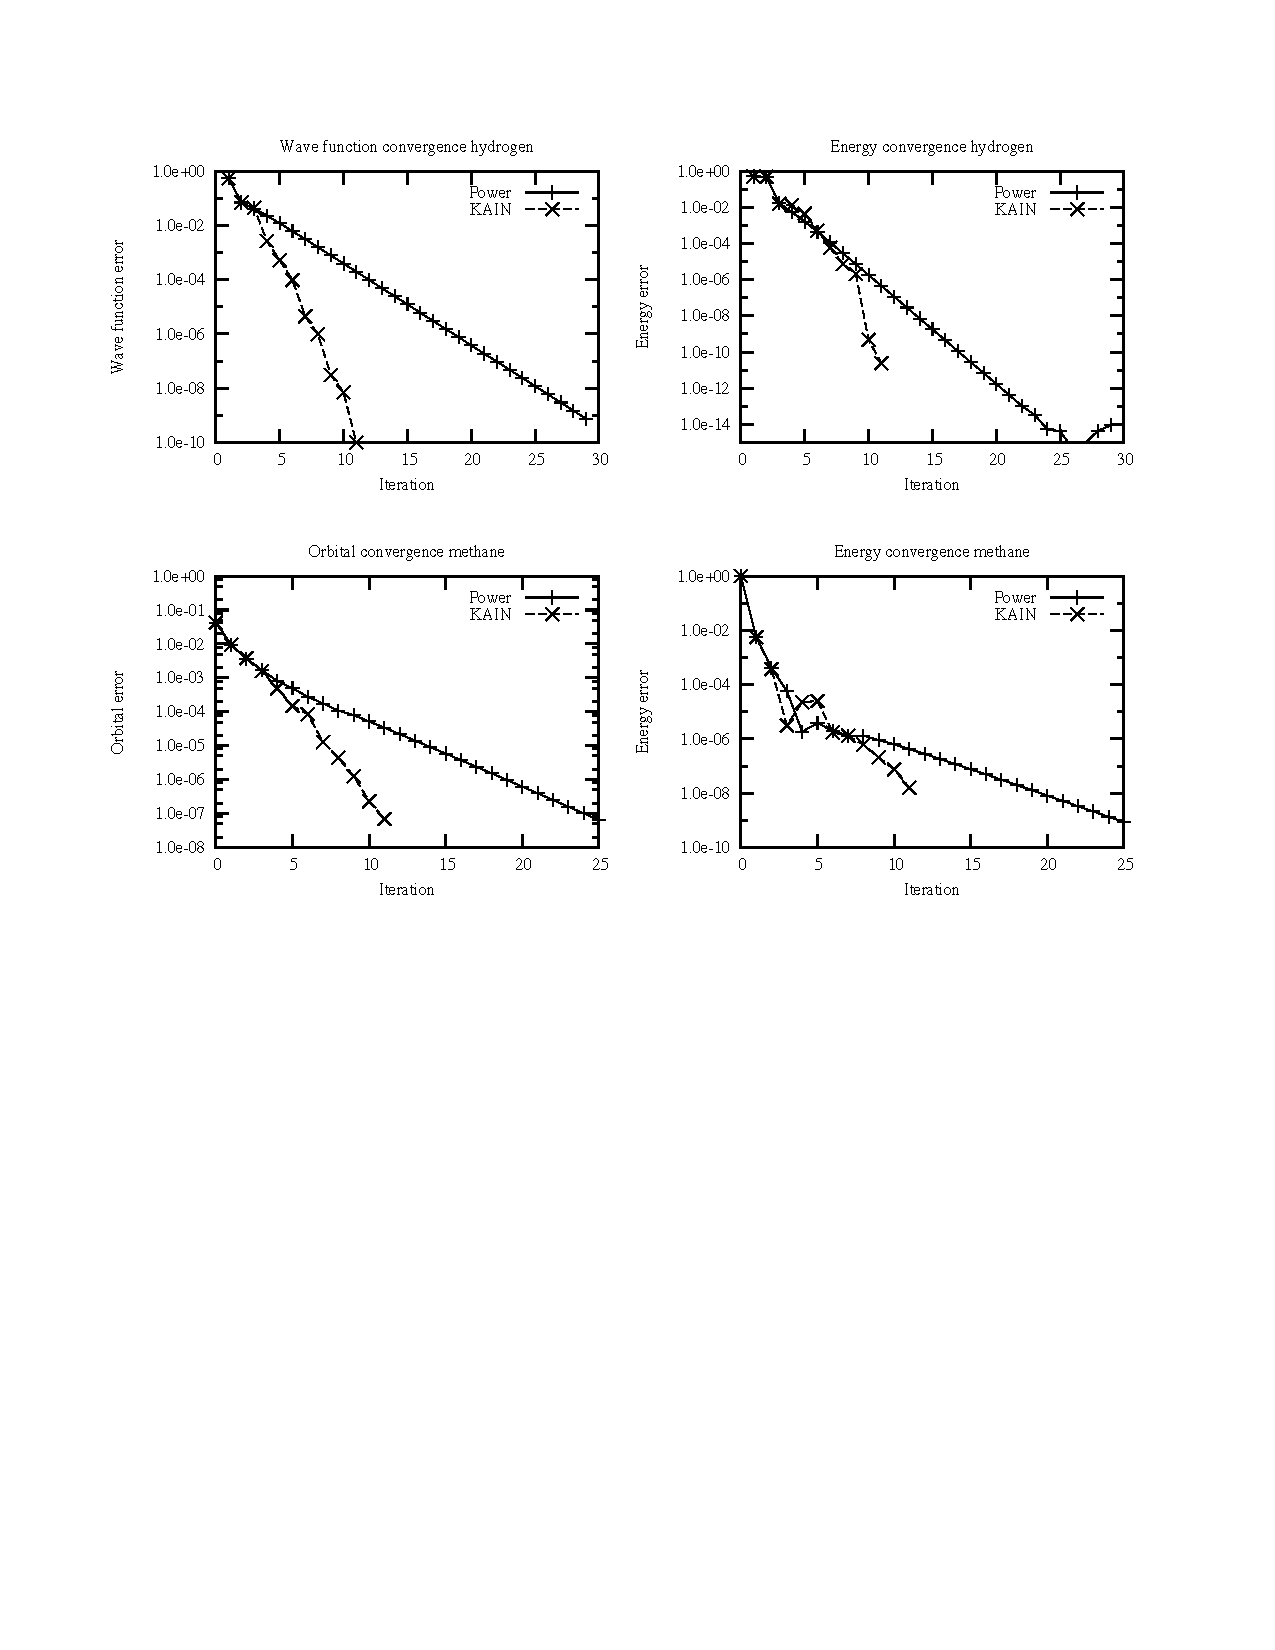
\includegraphics[scale=0.6, clip, viewport = 50 350 550 540]{figures/convergence.pdf}
    \end{center}
\end{frame}

\begin{frame}
    \frametitle{Many-electron systems}
    \centering
    Overall accuracy kept at $\epsilon = 10^{-6}$
    \begin{center}
	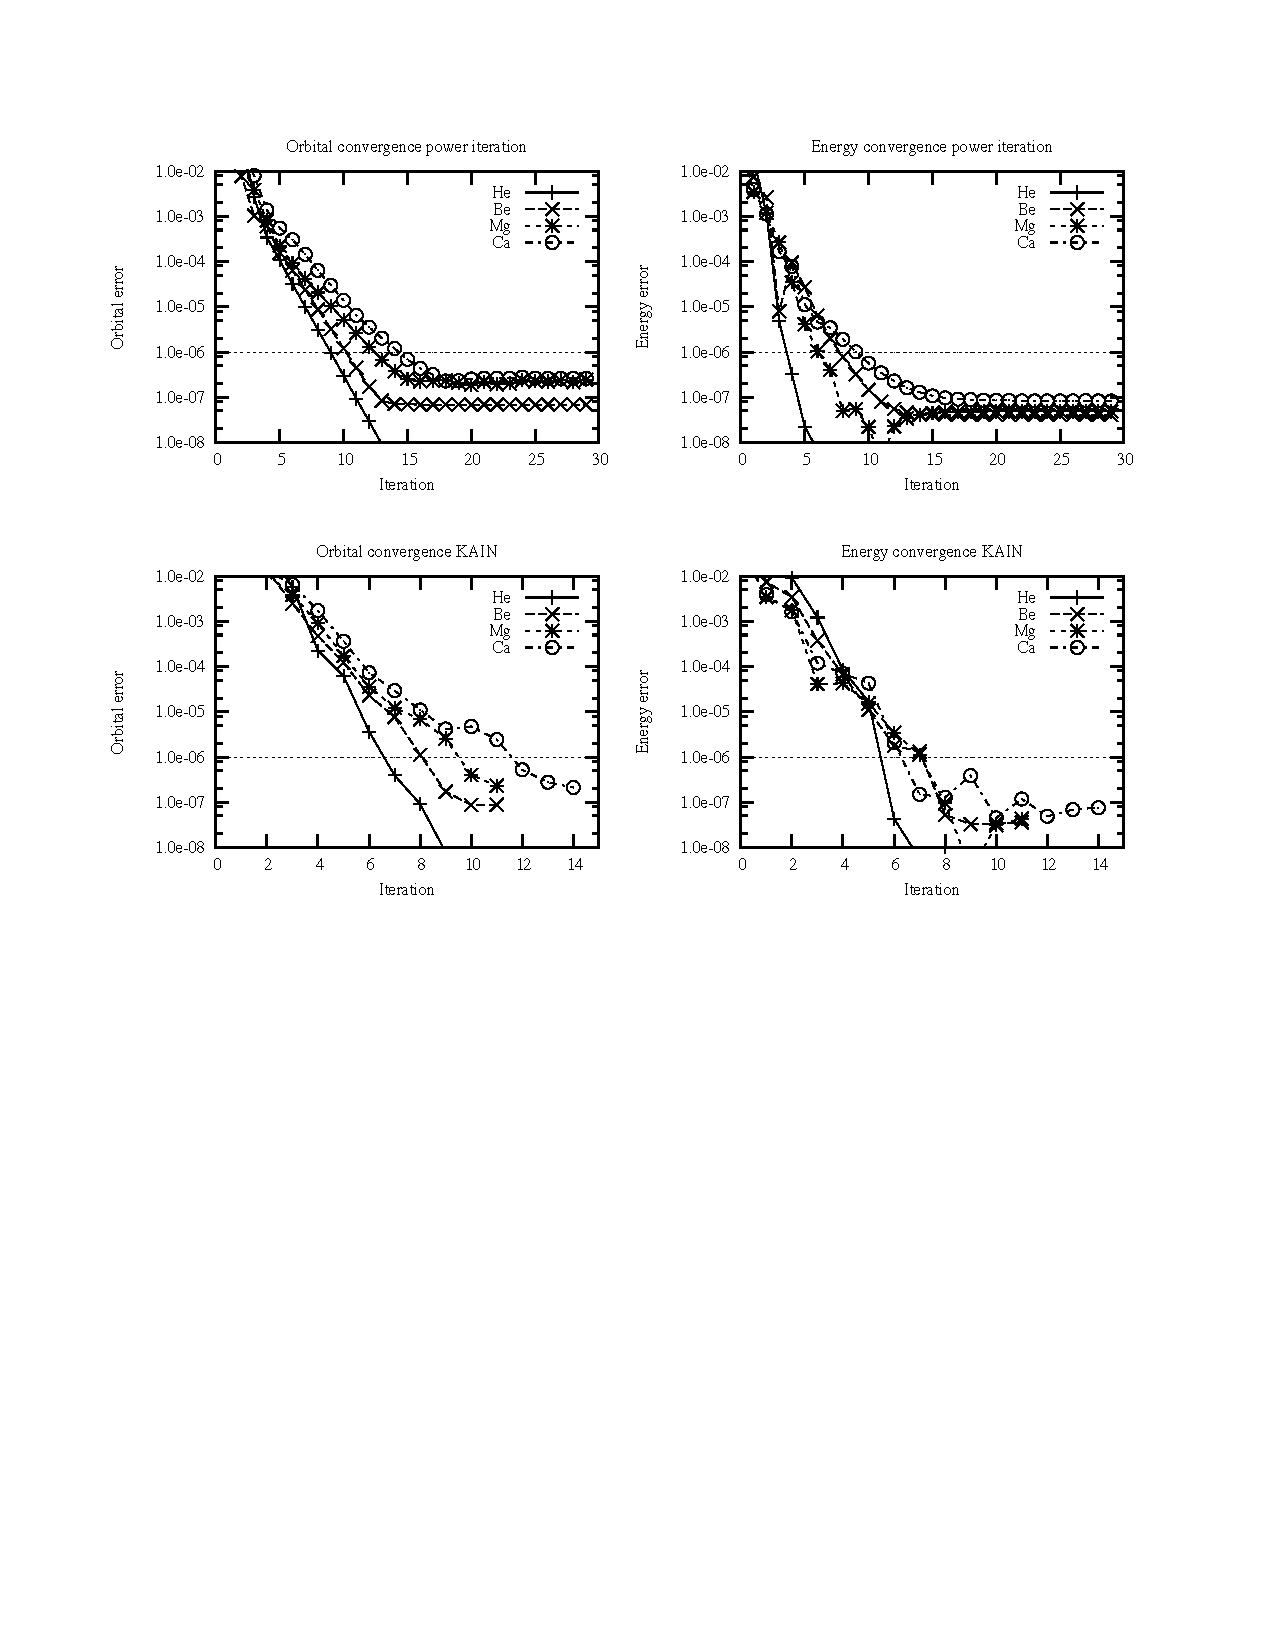
\includegraphics[scale=0.6, clip, viewport = 50 550 550 740]{figures/accuracy.pdf}
    \end{center}
    \ \\
    \ \\
    \ \\
    \begin{itemize}
        \item All orbitals of all atoms converge within the requested precision
        \item Energies are an order of magnitude more accurate than the orbitals
    \end{itemize}
\end{frame}

\begin{frame}
    \frametitle{Accurate calculations}
    \centering
    LDA energies in atomic units (Hartree)
    \begin{table}
	\tiny
	\centering
        \begin{tabular}{lr@{.}lr@{.}lr@{.}lr@{.}lr@{.}lr@{.}l}
	    \hline
	    \hline
	    &
	    \multicolumn{4}{c}{Helium}&\multicolumn{4}{c}{Neon}&\multicolumn{4}{c}{Argon}\\
	    &
	    \multicolumn{2}{c}{HOMO}&\multicolumn{2}{c}{Total}&
	    \multicolumn{2}{c}{HOMO}&\multicolumn{2}{c}{Total}&
	    \multicolumn{2}{c}{HOMO}&\multicolumn{2}{c}{Total}\\
	    \hline
	    &\multicolumn{4}{c}{}&\multicolumn{4}{c}{}&\multicolumn{4}{c}{}\\
	    MRChem $\epsilon=10^{-3}$&	-0&570467&-2&8348568&-0&496833&-128&262186&-0&387692&-525&966790\\
	    MRChem $\epsilon=10^{-5}$&	-0&570424&-2&8348352&-0&498035&-128&233472&-0&382348&-525&946109\\
	    MRChem $\epsilon=10^{-7}$&	-0&570425&-2&8348836&-0&498034&-128&233481&-0&382330&-525&946196\\
	    &\multicolumn{4}{c}{}&\multicolumn{4}{c}{}&\multicolumn{4}{c}{}\\
	    NIST&			-0&570425&-2&8348836&-0&498034&-128&233481&-0&382330&-525&946195\\
	    &\multicolumn{4}{c}{}&\multicolumn{4}{c}{}&\multicolumn{4}{c}{}\\
	    aug-cc-pV6Z&		-0&570424&-2&8348289&-0&498027&-128&233402&-0&382323&-525&944181\\
	    aug-cc-pV5Z&		-0&570417&-2&8347859&-0&498059&-128&232889&-0&382388&-525&942021\\
	    aug-cc-pVQZ&		-0&570406&-2&8346891&-0&498302&-128&229212&-0&382463&-525&938021\\
	    aug-cc-pVTZ&		-0&570260&-2&8343489&-0&498859&-128&218459&-0&382838&-525&933682\\
	    aug-cc-pVDZ&		-0&569386&-2&8291516&-0&498201&-128&176831&-0&382143&-525&915702\\
	    &\multicolumn{4}{c}{}&\multicolumn{4}{c}{}&\multicolumn{4}{c}{}\\
	    \hline
	    \hline
	\end{tabular}
    \end{table}
    \it{NIST: National Institute of Standards and Technology (Basis set limit)}\\
\ \\
\ \\
\ \\
\begin{itemize}
    \item We are able to attain \textbf{considerably higher} accuracy than high-quality Gaussian basis sets
    \item Energies are not variational, but \textbf{basis set limit} within the requested precision
    \item Calculations are still more expensive than conventional methods
\end{itemize}
\end{frame}

\begin{frame}
    \frametitle{Orbital localization}
    \centering
    Total energy invariant under unitary transformations among occupied orbitals
    \begin{equation}
	\nonumber
	\phi_i(\boldsymbol{r}) = \sum_j U_{ji}^\ast \phi_i(\boldsymbol{r}), \qquad \qquad U^\ast U = UU^\ast = I
    \end{equation}
    Possible to find matrix $U$ that leads to localized orbitals\\
    \begin{columns}
    \begin{column}[b]{0.48\linewidth}
    \begin{center}
	\only<1>{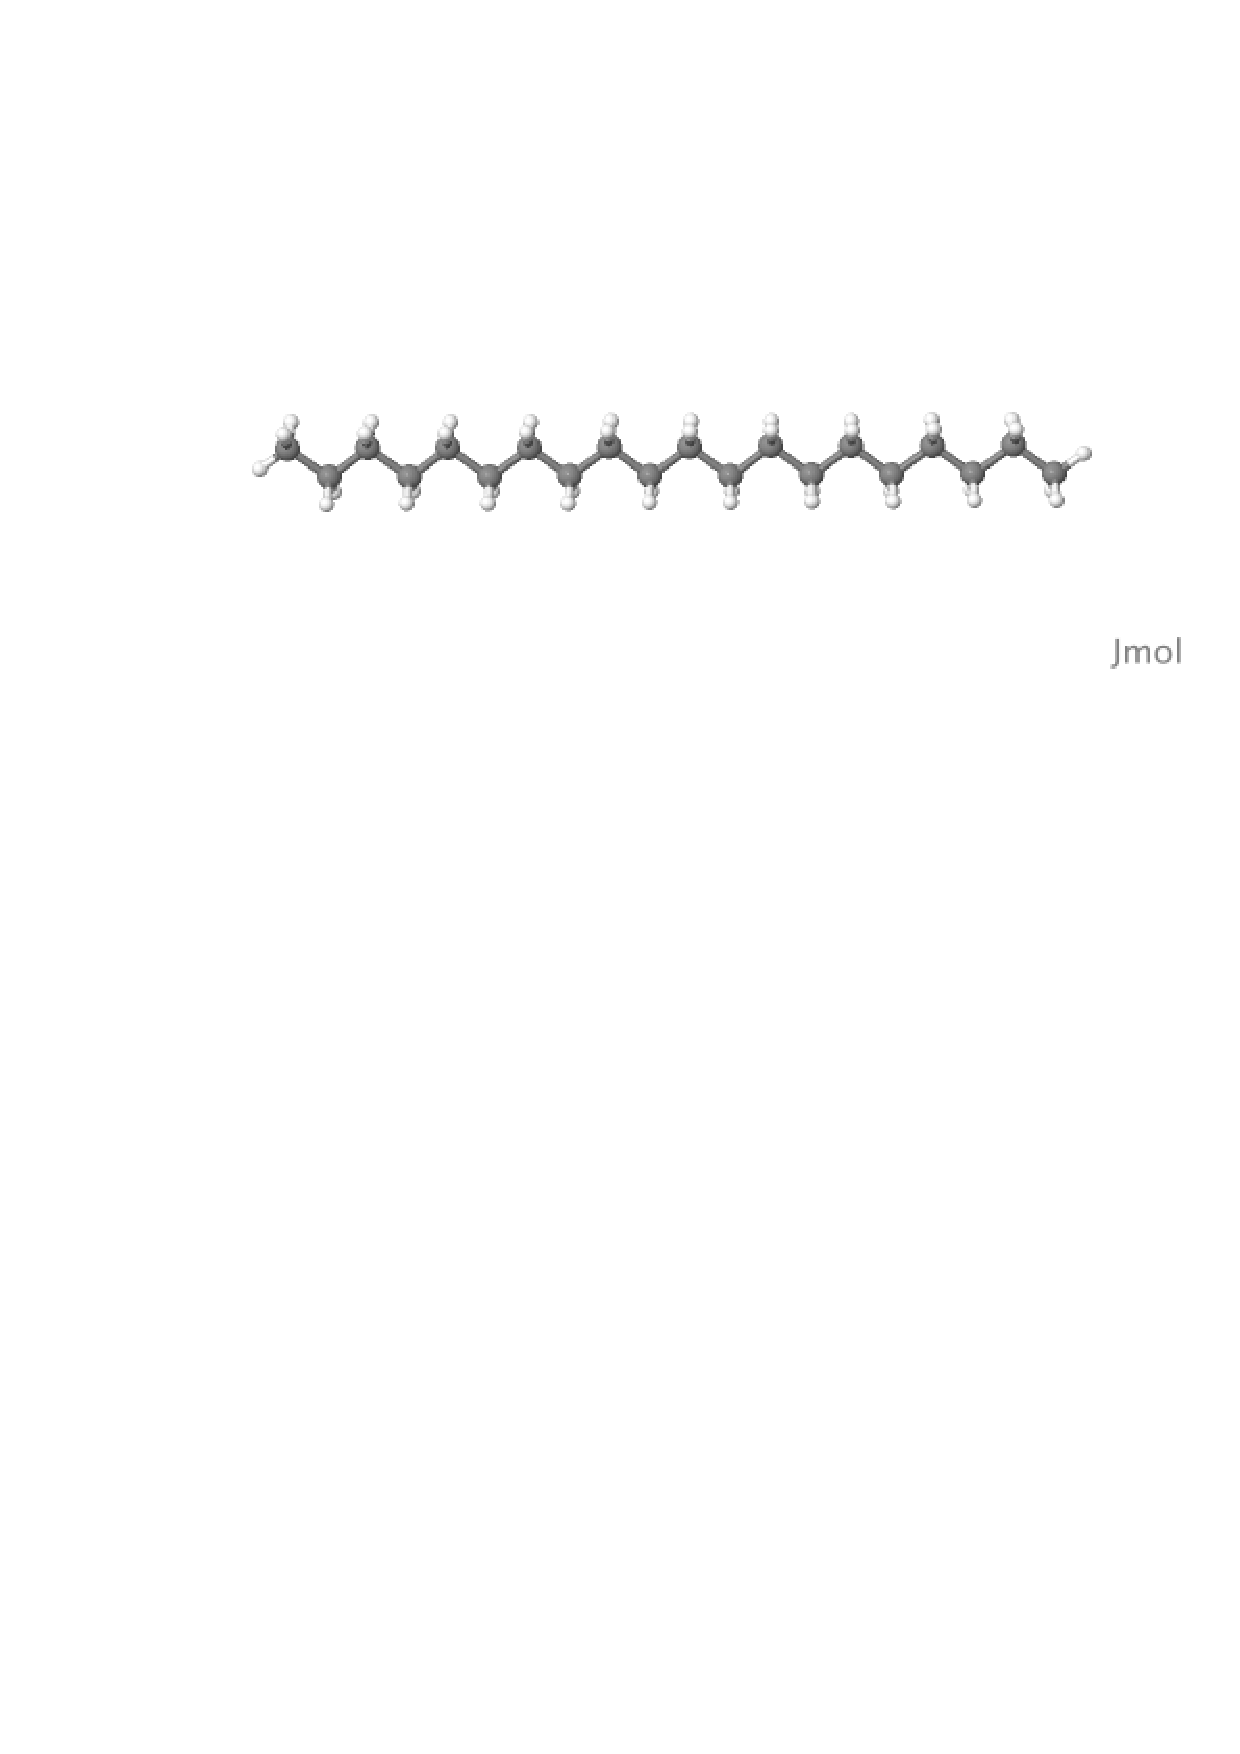
\includegraphics[scale=0.3, clip, viewport = 80 260 600 400]{figures/alkane.pdf}}
	\only<2,3>{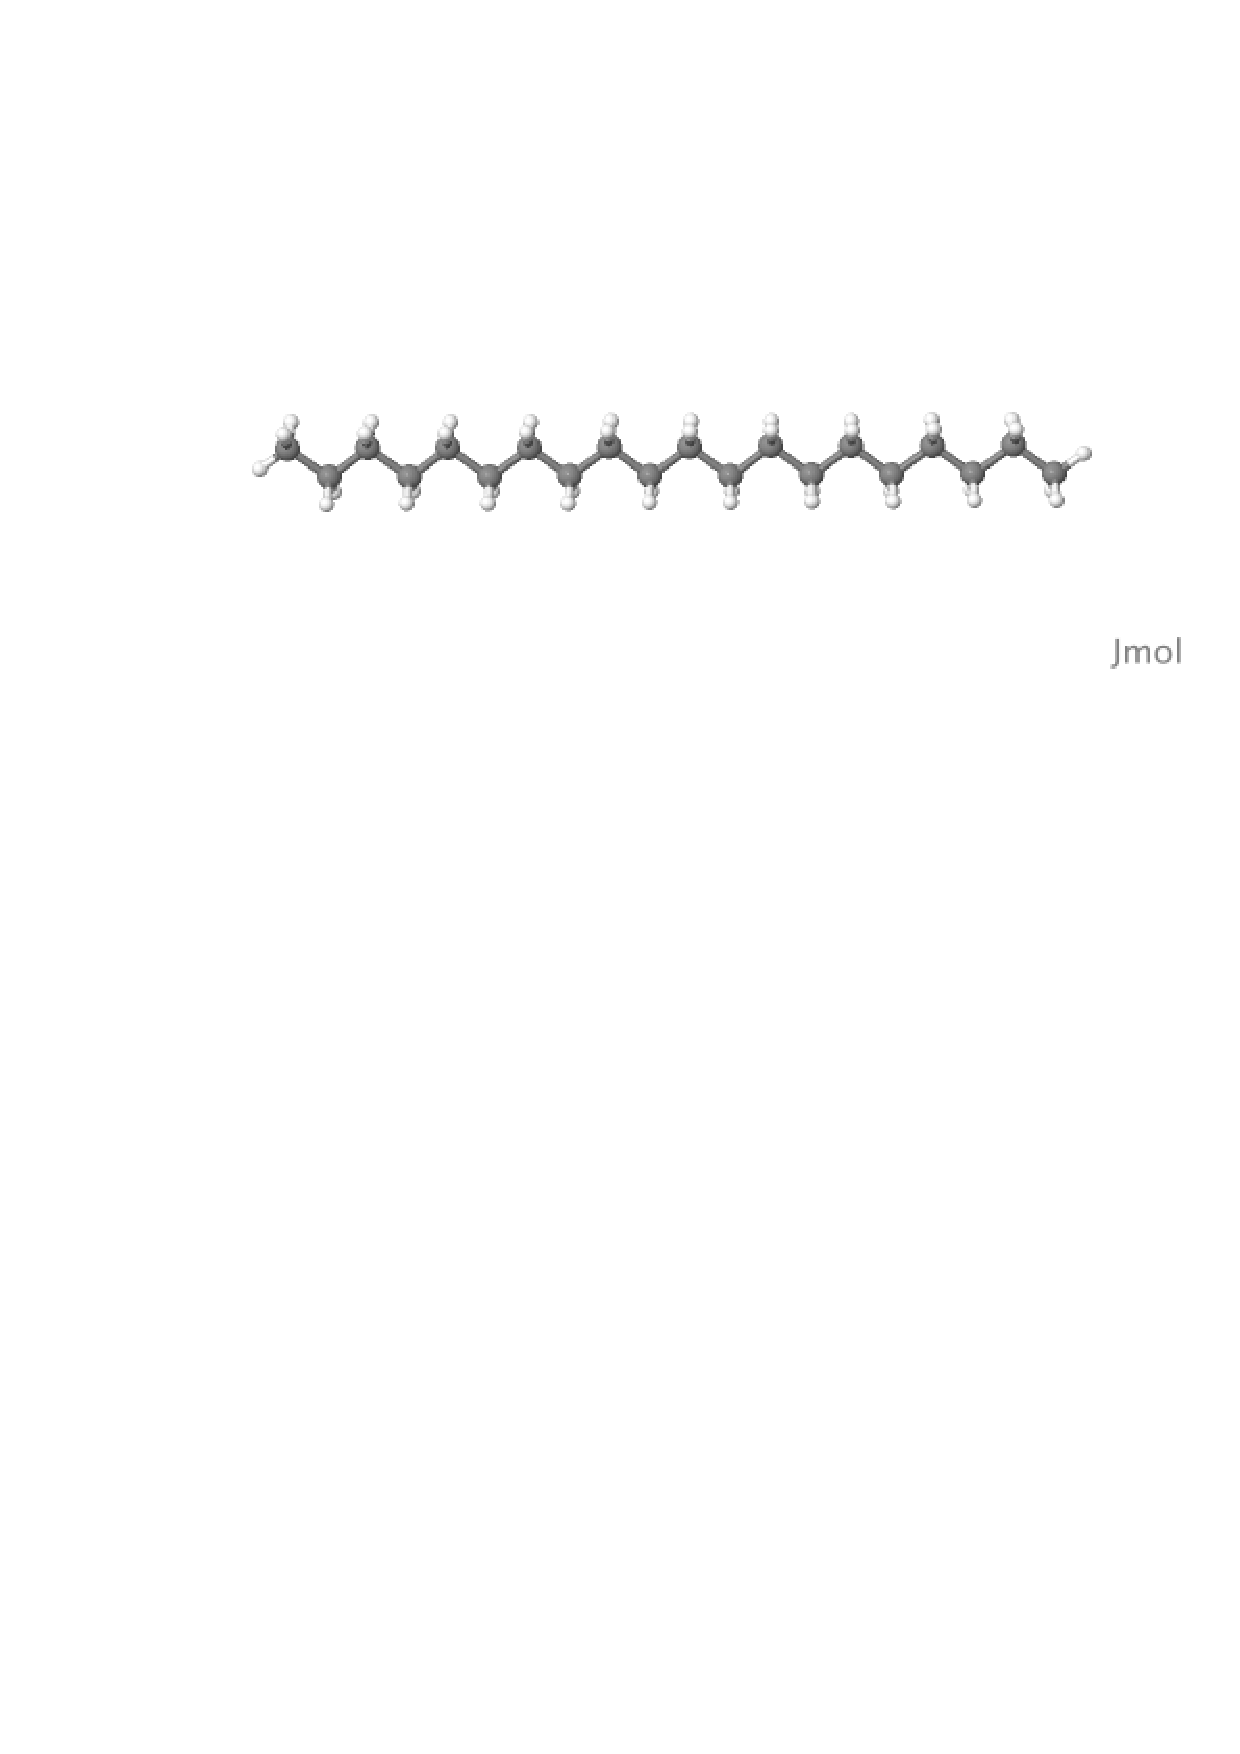
\includegraphics[scale=0.3, clip, viewport = 80 560 600 700]{figures/alkane.pdf}}
	\only<1>{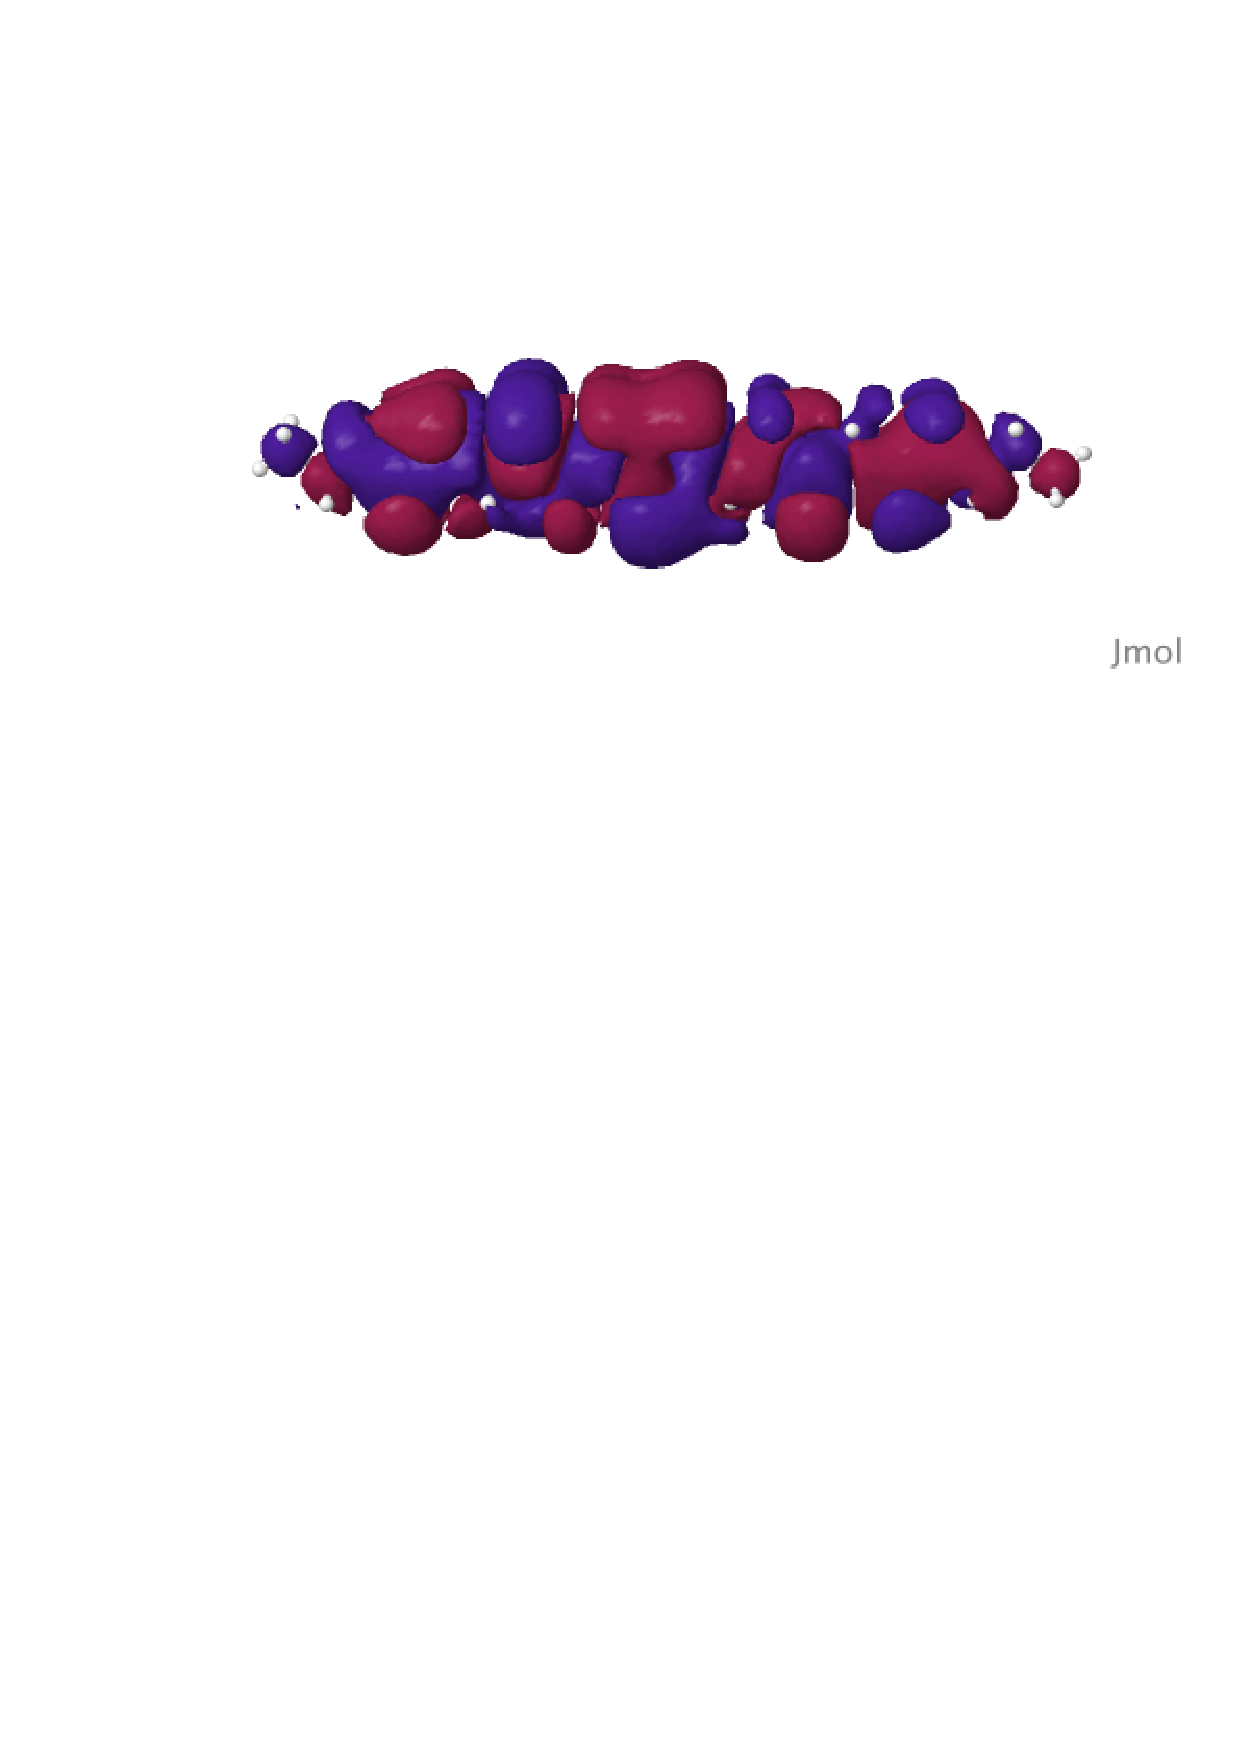
\includegraphics[scale=0.3, clip, viewport = 80 260 600 400]{figures/can_orb_1.pdf}}
	\only<2,3>{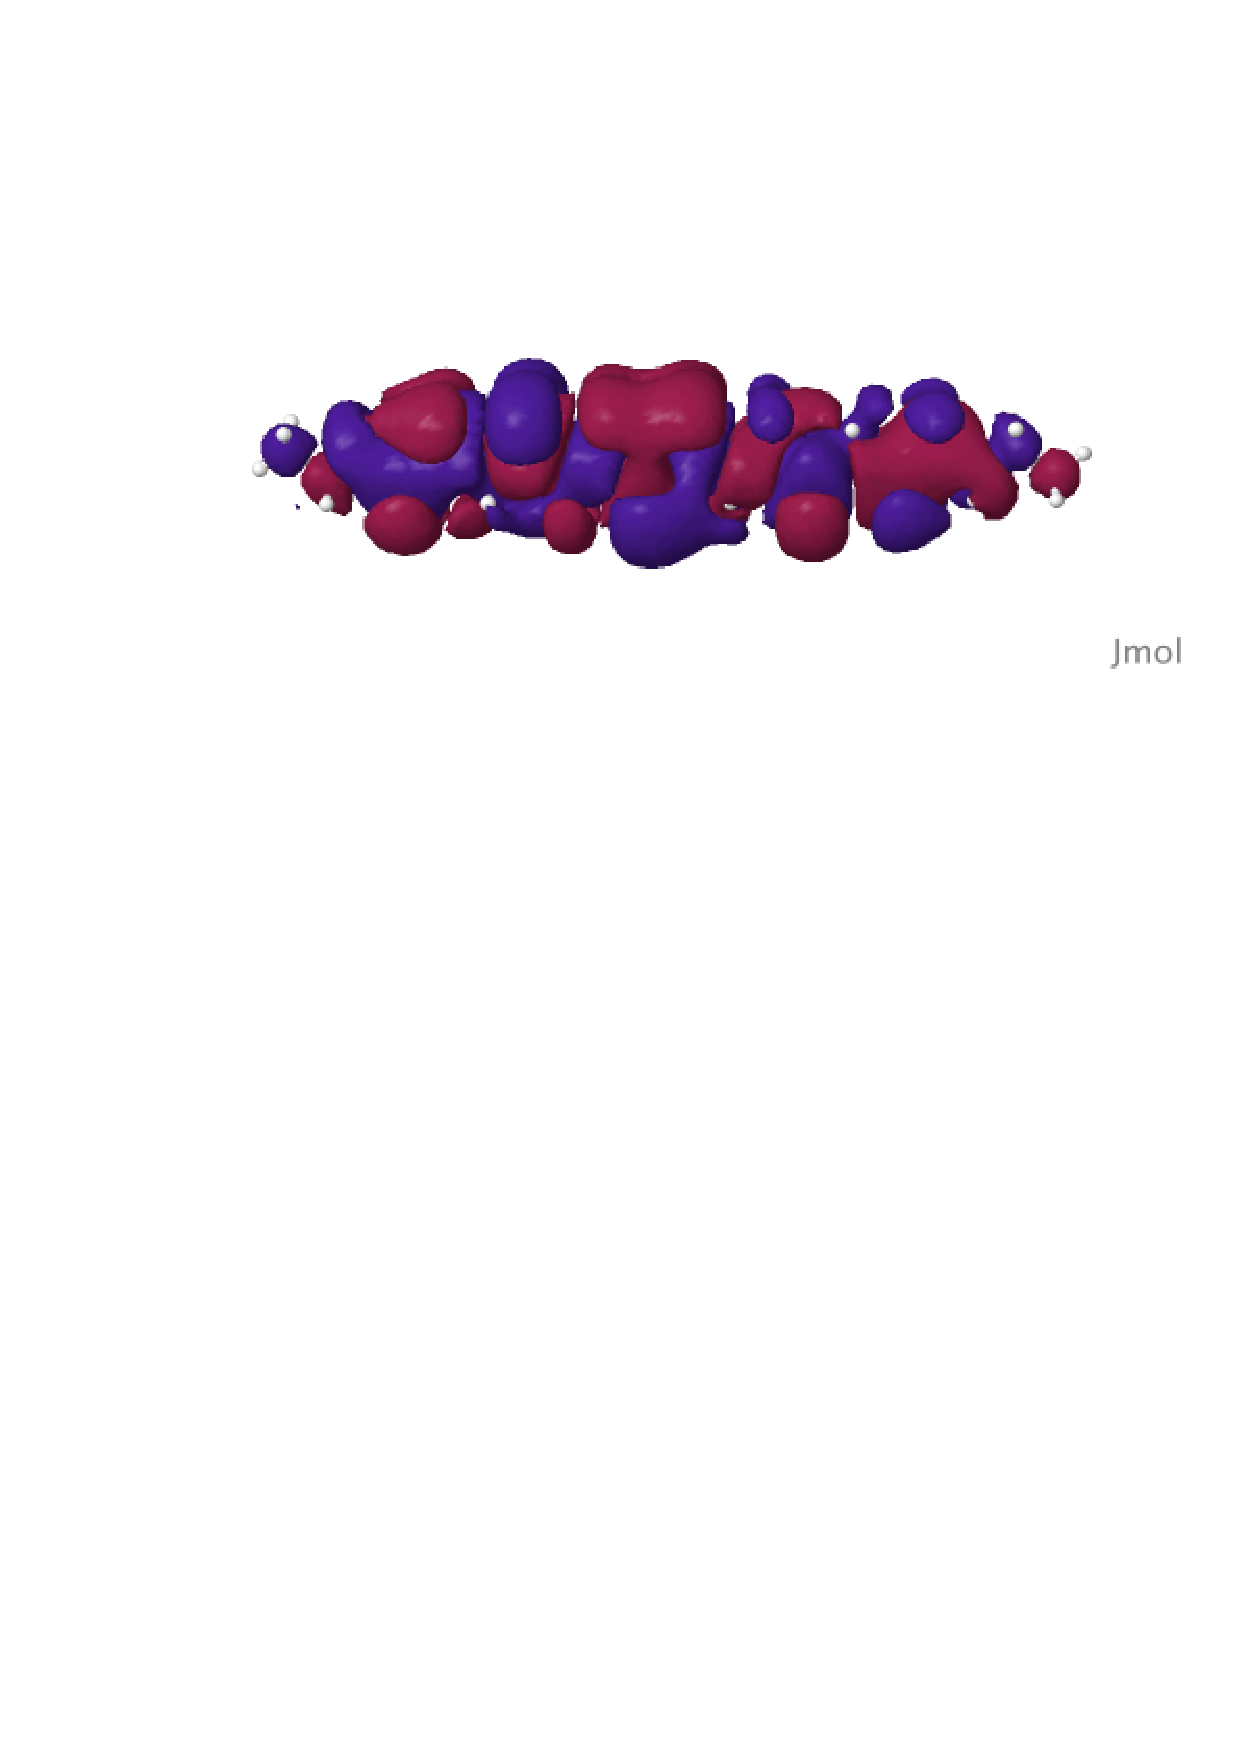
\includegraphics[scale=0.3, clip, viewport = 80 560 600 700]{figures/can_orb_1.pdf}}
	\only<1>{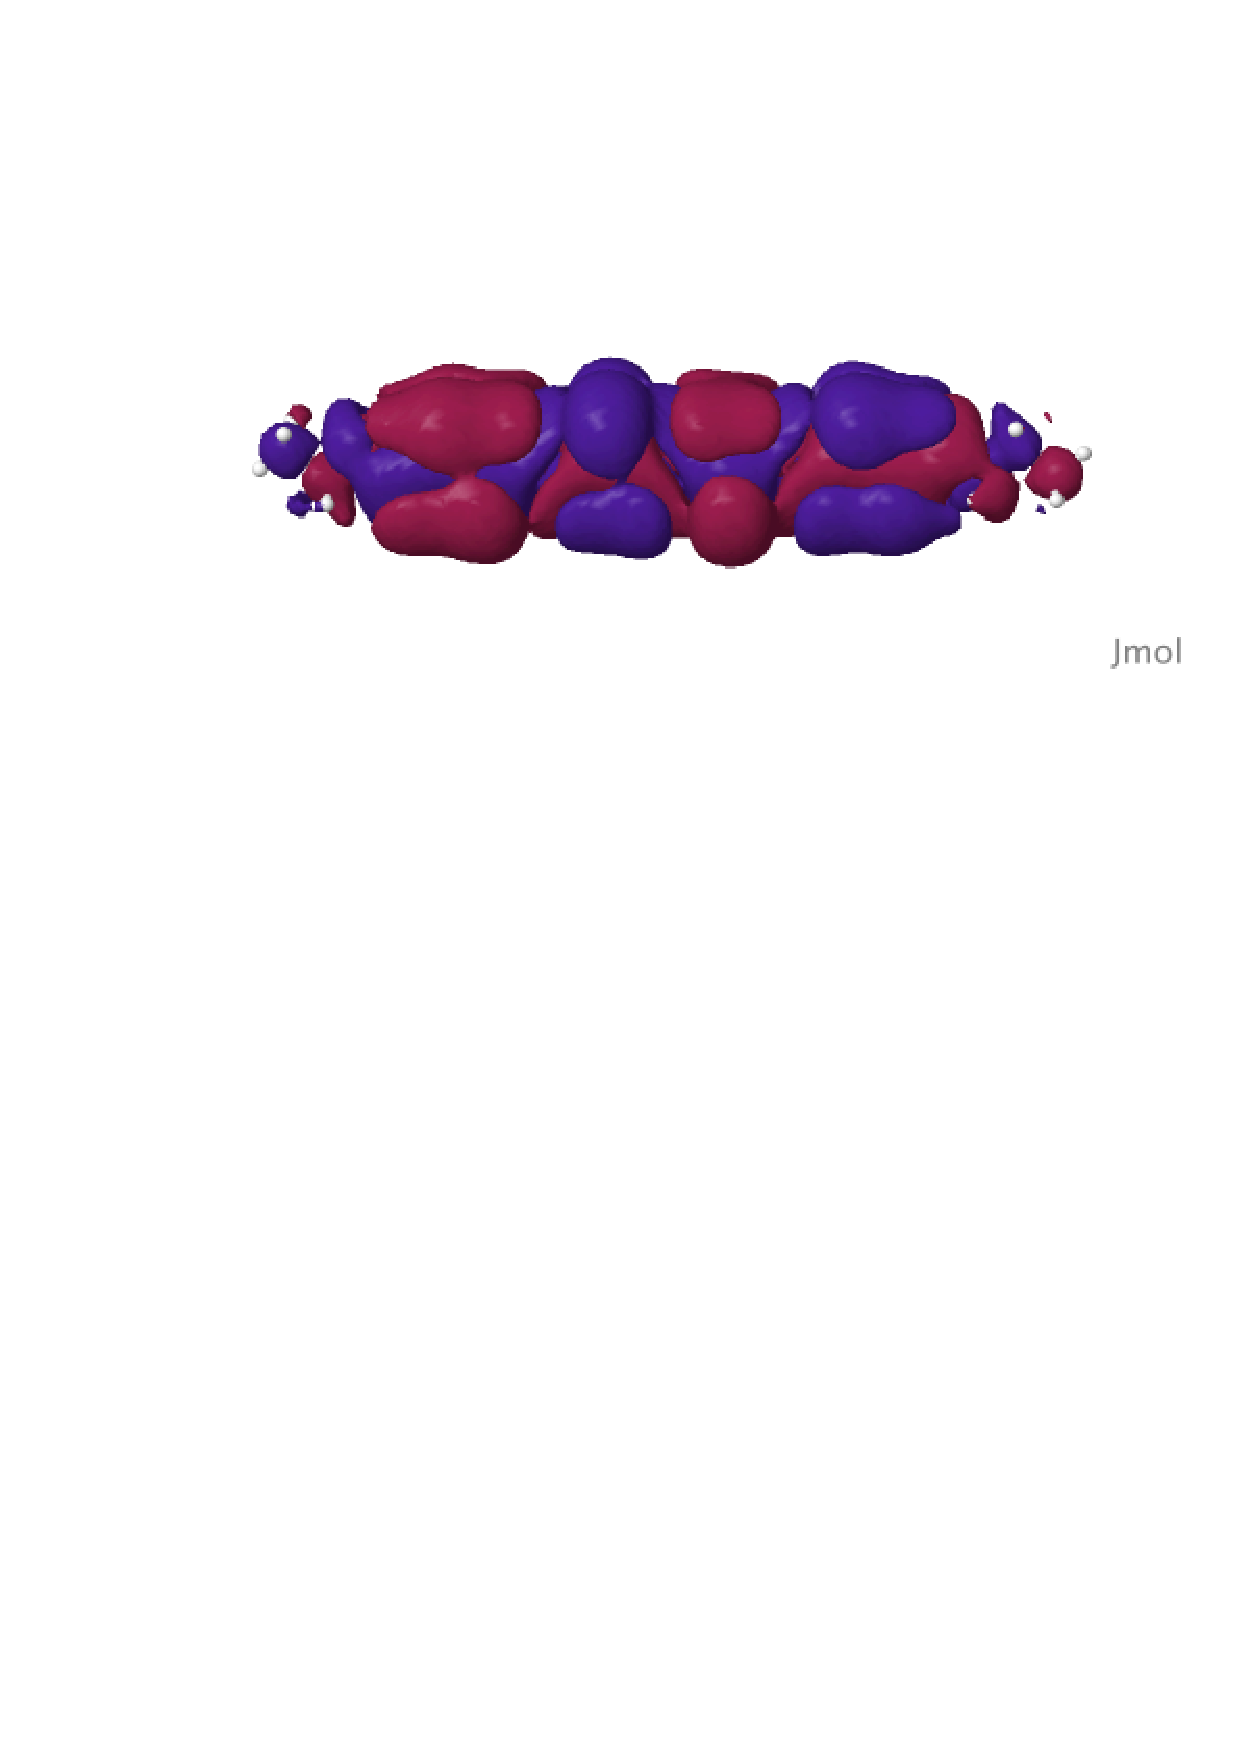
\includegraphics[scale=0.3, clip, viewport = 80 260 600 400]{figures/can_orb_2.pdf}}
	\only<2,3>{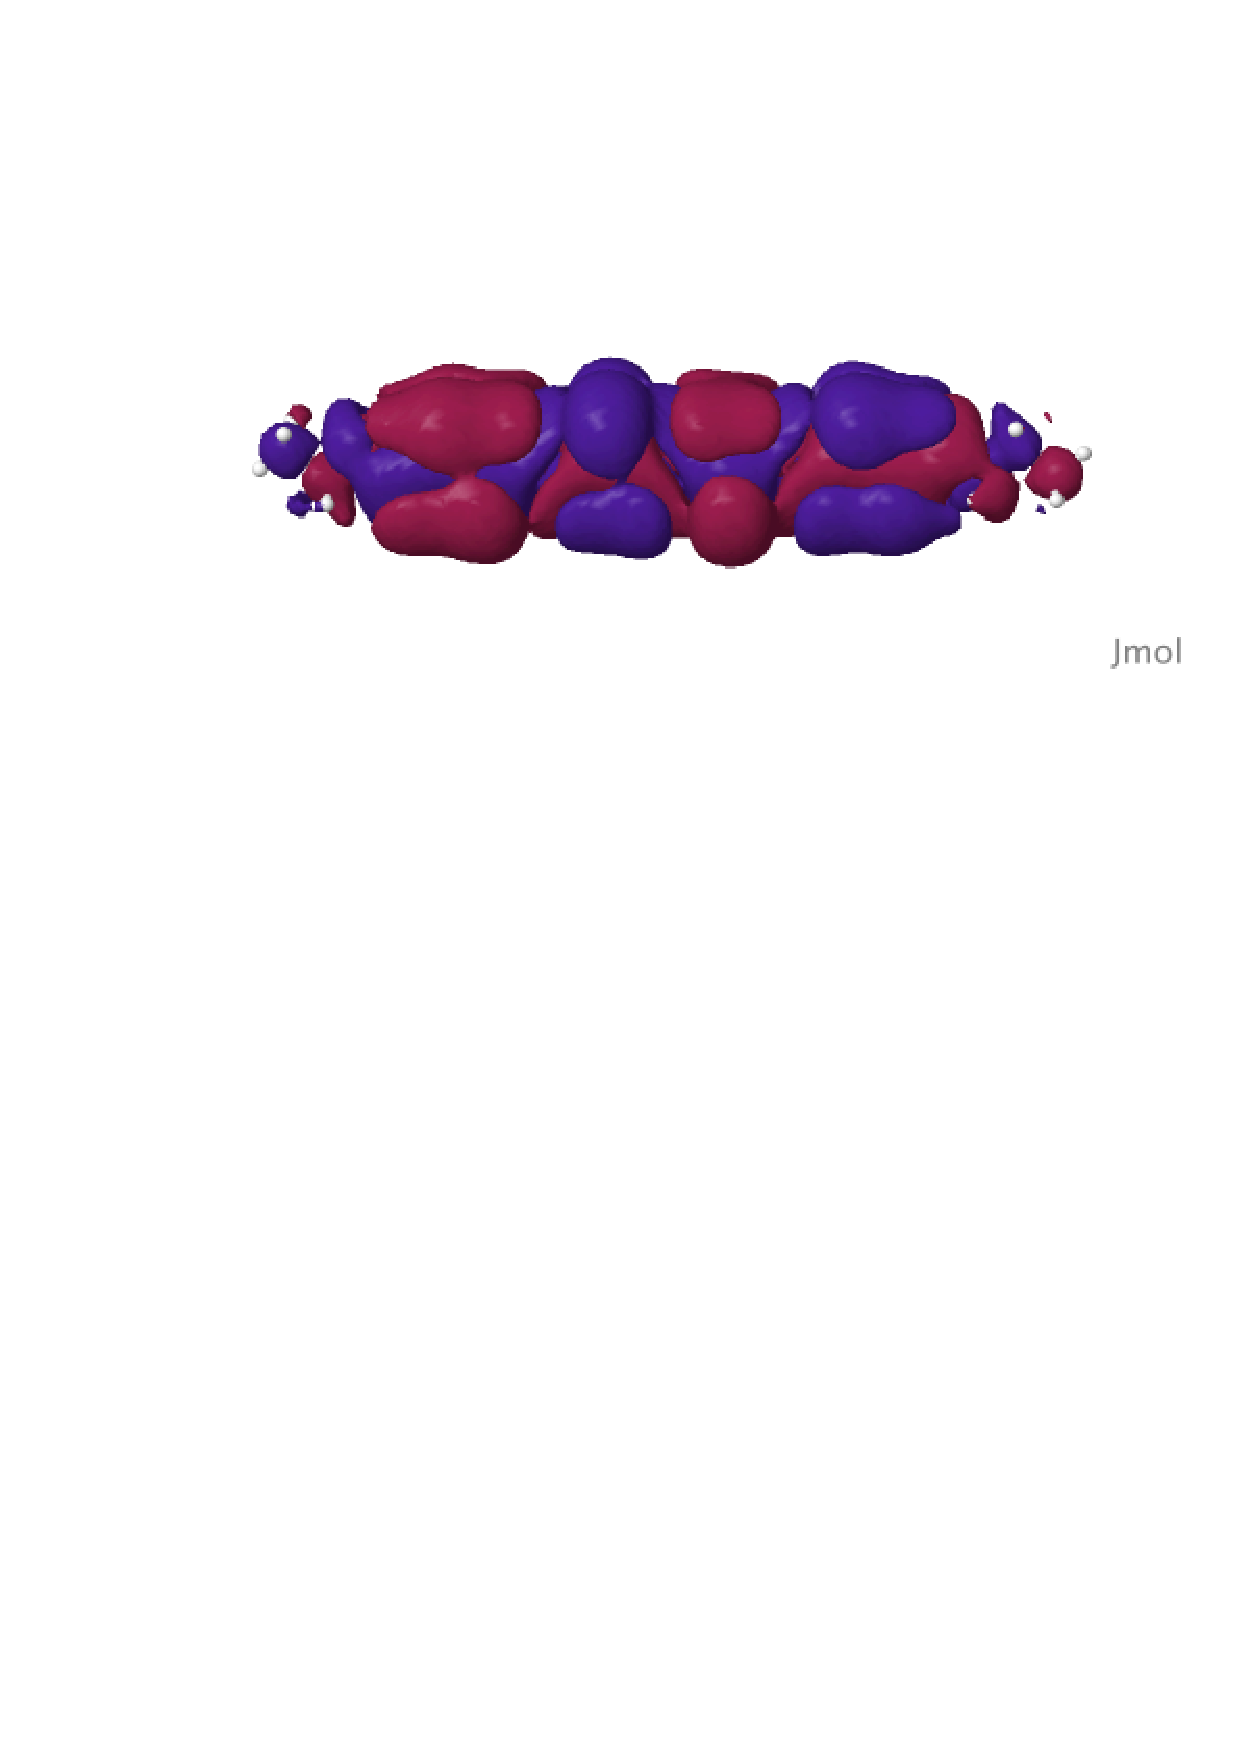
\includegraphics[scale=0.3, clip, viewport = 80 560 600 700]{figures/can_orb_2.pdf}}
    \end{center}
    \end{column}
    \begin{column}[b]{0.48\linewidth}
    \begin{center}
	\only<3>{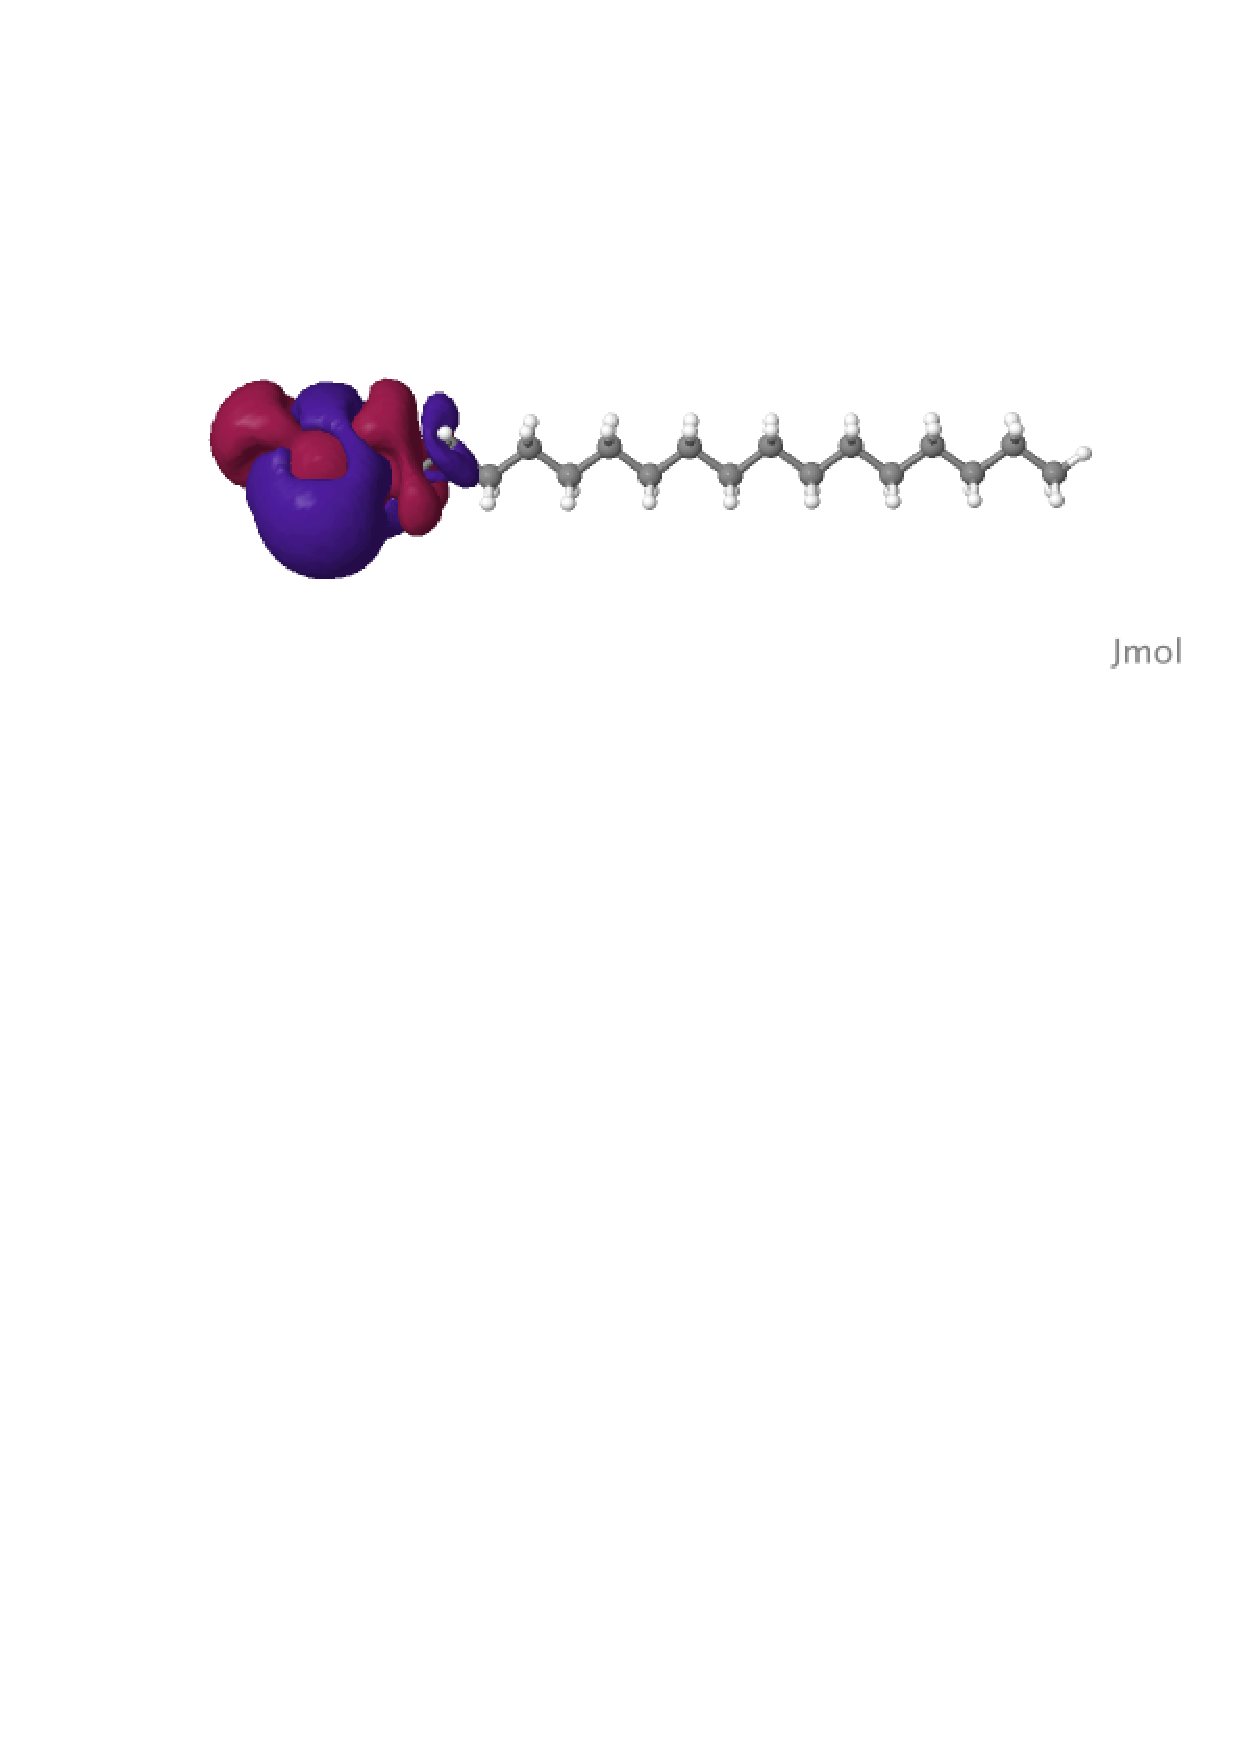
\includegraphics[scale=0.3, clip, viewport = 80 560 600 700]{figures/loc_orb_1.pdf}\\}
	\only<3>{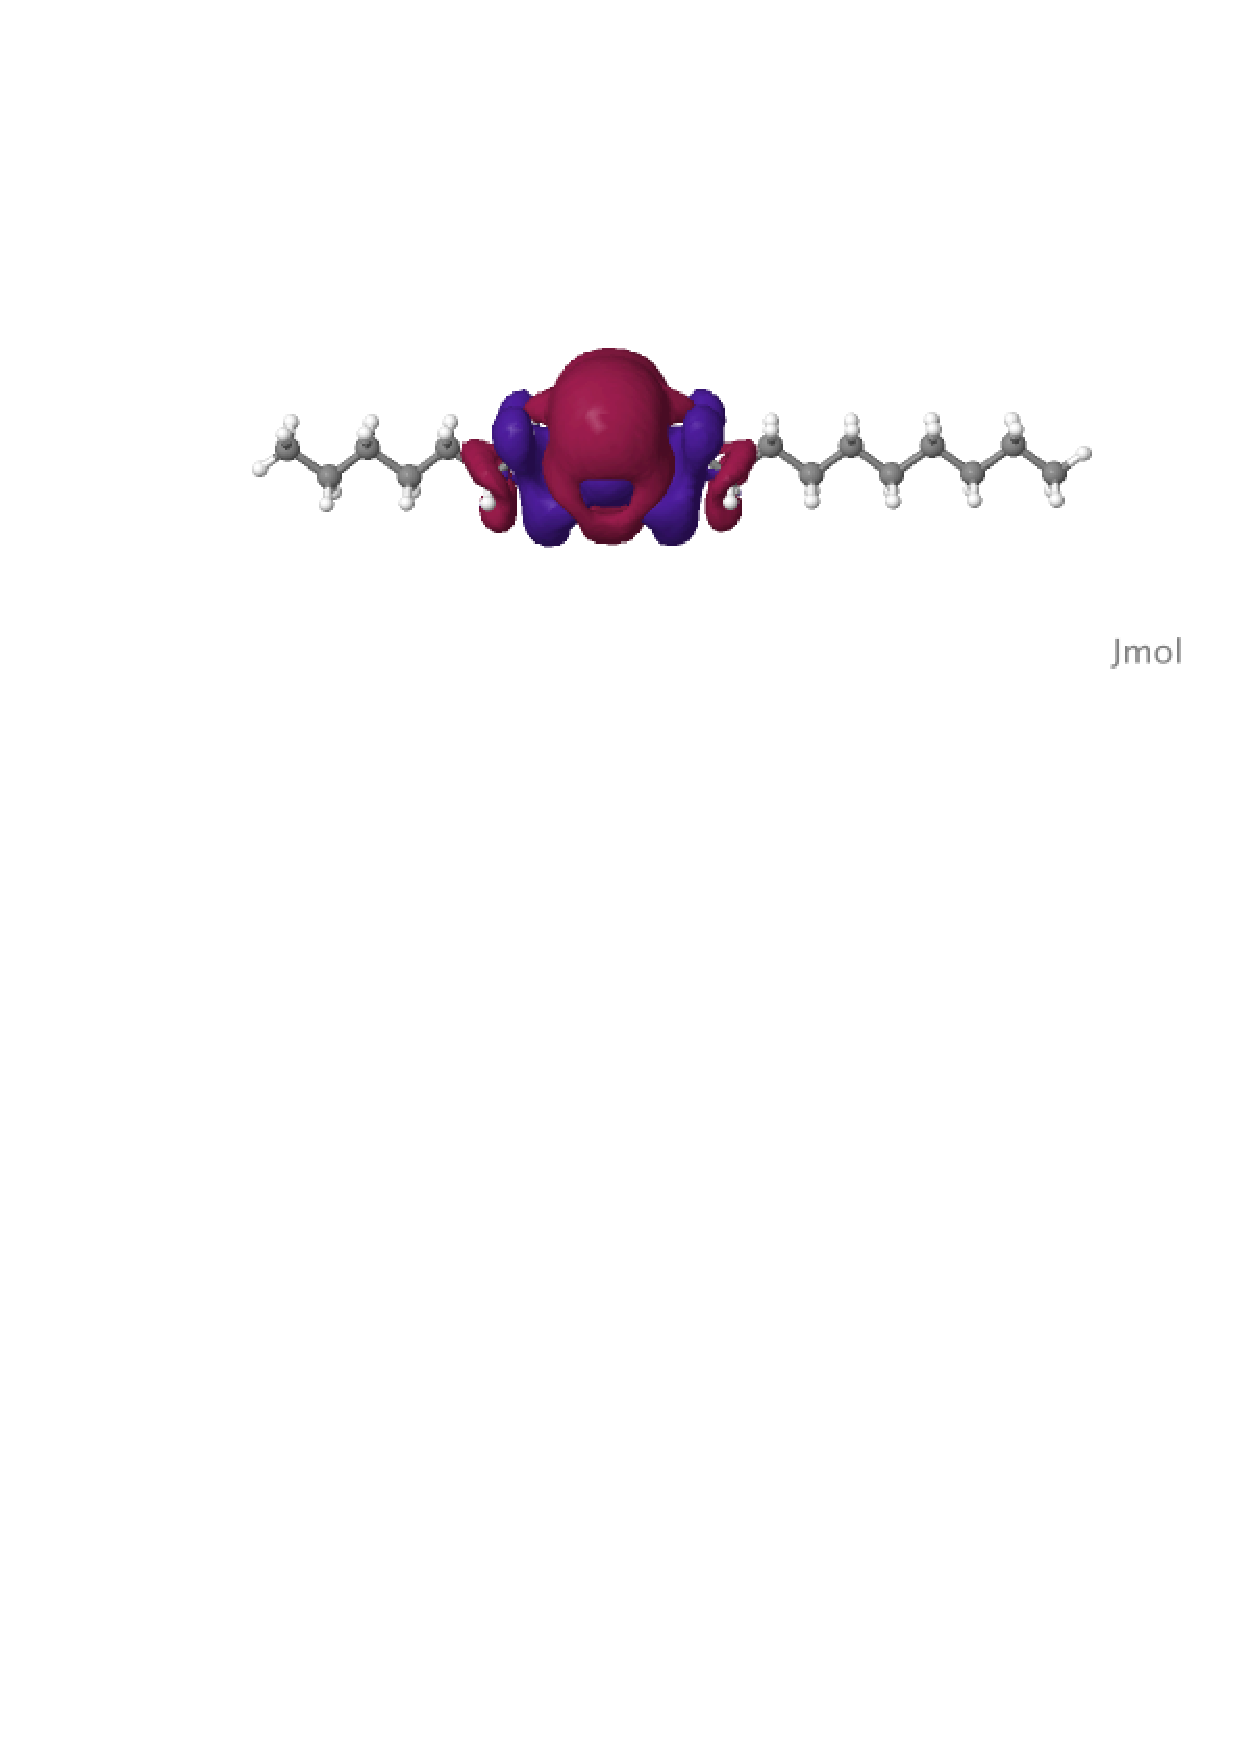
\includegraphics[scale=0.3, clip, viewport = 80 560 600 700]{figures/loc_orb_2.pdf}\\}
	\only<3>{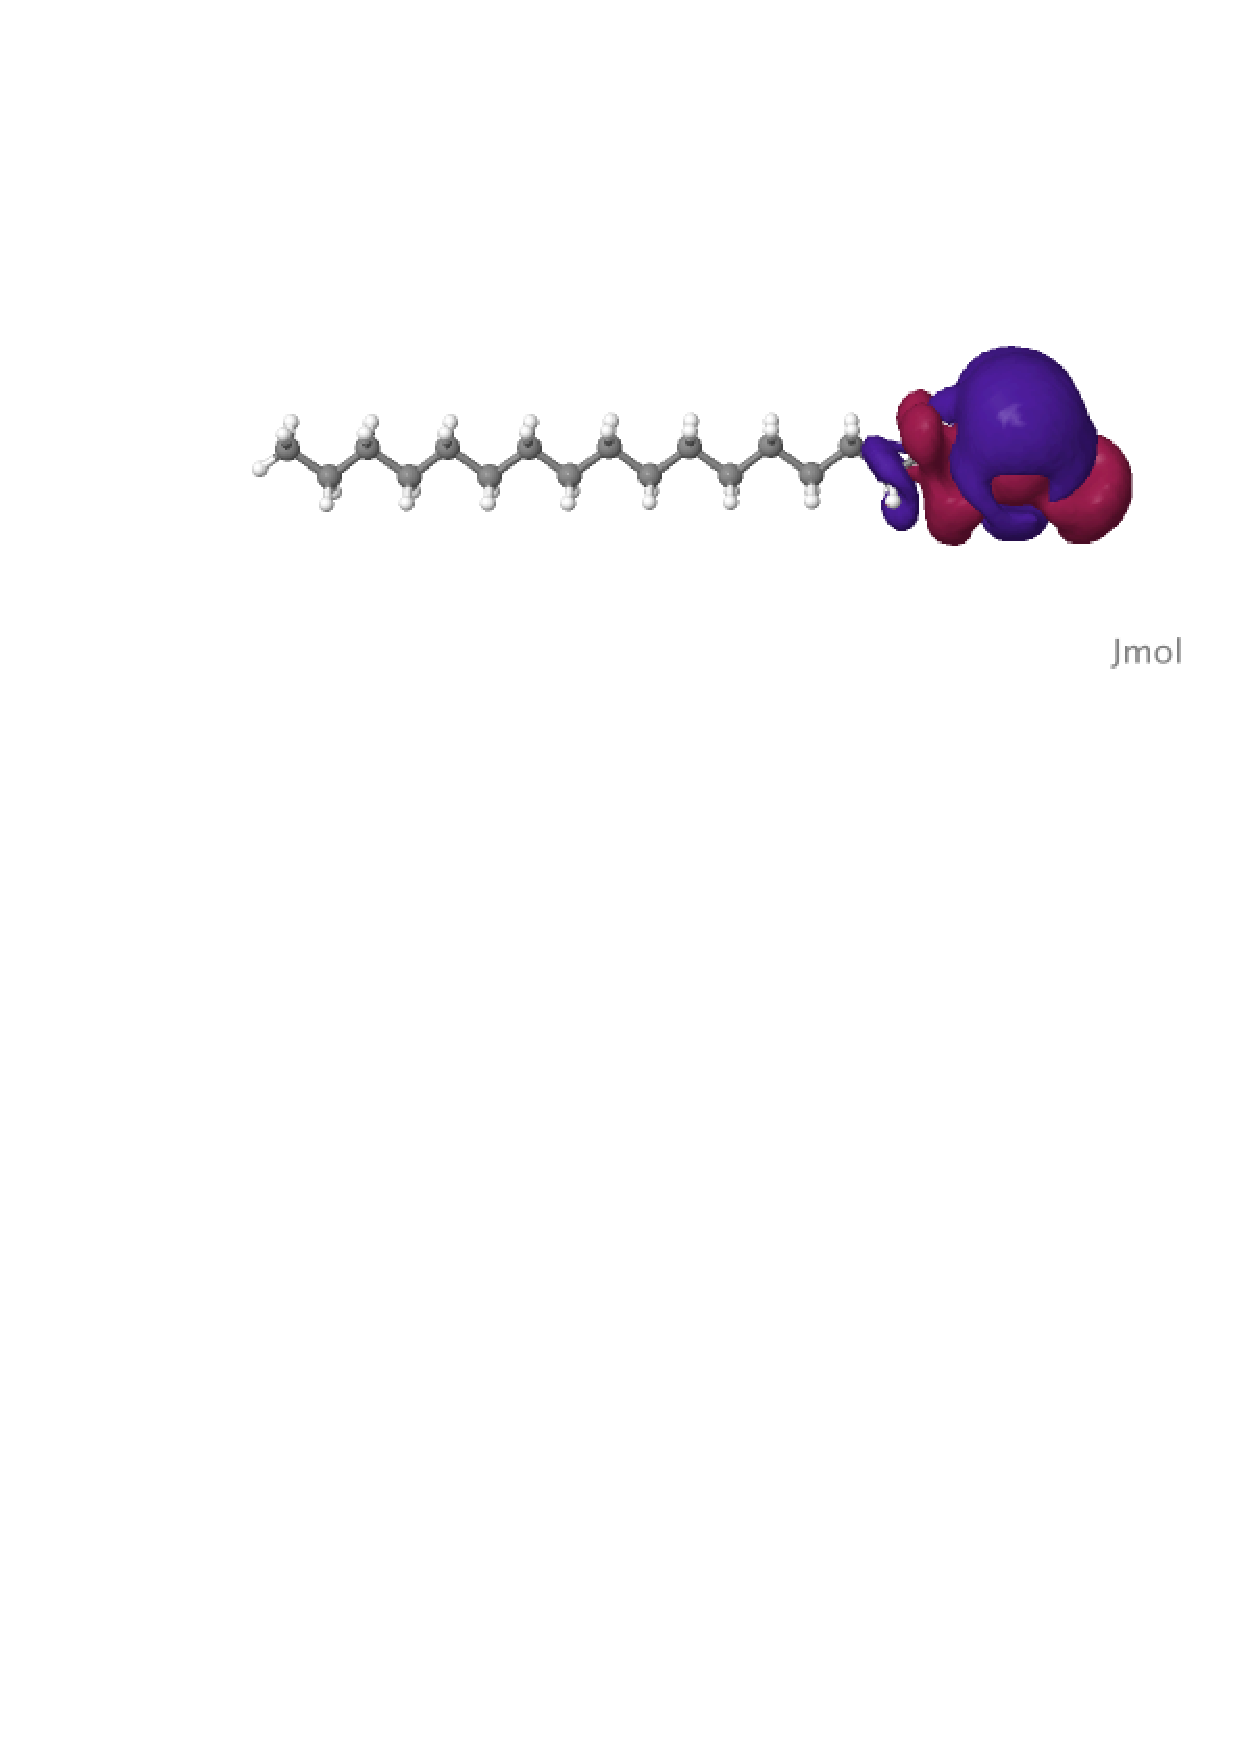
\includegraphics[scale=0.3, clip, viewport = 80 560 600 700]{figures/loc_orb_3.pdf}}
    \end{center}
    \end{column}
    \end{columns}
\end{frame}

\begin{frame}
    \frametitle{Accurate calculations}
    \centering
    Replacing the exchange-correlation potential $v_{xc}$ with the exact exchange operator
    \begin{equation}
	\nonumber
	\hat{K}\phi_i(\boldsymbol{r}) = \sum_j \phi_j(\boldsymbol{r}) \int P(\boldsymbol{r}-\boldsymbol{r}')
	    \left[\phi_i(\boldsymbol{r}')\phi_j(\boldsymbol{r}')\right] d\boldsymbol{r}'
    \end{equation}
    gives the Hartree-Fock equations, which can be solved by the same iterative methods
    \ \\
    \ \\
\begin{table}
\tiny
\begin{tabular}{cllll}
\hline   
\hline
\multicolumn{5}{c}{Total Hartree-Fock energies in atomic units (Hartree)}\\
&\multicolumn{1}{c}{H$_2$O}
&\multicolumn{1}{c}{H$_2$O$_2$}
&\multicolumn{1}{c}{CO}
&\multicolumn{1}{c}{CO$_2$}\\
\hline 
            		    &               &               &               &               \\
MRChem $\epsilon=10^{-5}$   & -76.067611455 & -150.85253297 & -112.79087294 & -187.72538886 \\
MRChem $\epsilon=10^{-6}$   & -76.067556696 & -150.85249254 & -112.79069389 & -187.72541991 \\
MRChem $\epsilon=10^{-7}$   & -76.067535613 & -150.85246986 & -112.79081263 & -187.72538522 \\
MRChem $\epsilon=10^{-8}$   & -76.067535431 & -150.85247037 & -112.79081269 & -187.72538560 \\
            		    &               &               &               &               \\
Est. HF limit		    & -76.0675      & -150.8525     & -112.7908     & -187.7254     \\
            		    &               &               &               &               \\
aug-cc-pCV5Z		    & -76.067379371 & -150.85218780 & -112.79063514 & -187.72508317 \\
aug-cc-pCVQZ		    & -76.066140457 & -150.84985235 & -112.78919290 & -187.72260431 \\
            		    &               &               &               &               \\
\hline   
\hline   
\end{tabular}
\end{table}
\ \\
\ \\
\ \\
\begin{itemize}
    \item We are able to attain \textbf{considerably higher} accuracy than high-quality Gaussian basis sets
    \item Energies are not variational, but \textbf{basis set limit} within the requested precision
    \item Calculations are still more expensive than conventional methods
\end{itemize}
\end{frame}

\end{document}
